\documentclass[twoside]{book}

% Packages required by doxygen
\usepackage{fixltx2e}
\usepackage{calc}
\usepackage{doxygen}
\usepackage[export]{adjustbox} % also loads graphicx
\usepackage{graphicx}
\usepackage[utf8]{inputenc}
\usepackage{makeidx}
\usepackage{multicol}
\usepackage{multirow}
\PassOptionsToPackage{warn}{textcomp}
\usepackage{textcomp}
\usepackage[nointegrals]{wasysym}
\usepackage[table]{xcolor}

% Font selection
\usepackage[T1]{fontenc}
\usepackage[scaled=.90]{helvet}
\usepackage{courier}
\usepackage{amssymb}
\usepackage{sectsty}
\renewcommand{\familydefault}{\sfdefault}
\allsectionsfont{%
  \fontseries{bc}\selectfont%
  \color{darkgray}%
}
\renewcommand{\DoxyLabelFont}{%
  \fontseries{bc}\selectfont%
  \color{darkgray}%
}
\newcommand{\+}{\discretionary{\mbox{\scriptsize$\hookleftarrow$}}{}{}}

% Page & text layout
\usepackage{geometry}
\geometry{%
  a4paper,%
  top=2.5cm,%
  bottom=2.5cm,%
  left=2.5cm,%
  right=2.5cm%
}
\tolerance=750
\hfuzz=15pt
\hbadness=750
\setlength{\emergencystretch}{15pt}
\setlength{\parindent}{0cm}
\setlength{\parskip}{3ex plus 2ex minus 2ex}
\makeatletter
\renewcommand{\paragraph}{%
  \@startsection{paragraph}{4}{0ex}{-1.0ex}{1.0ex}{%
    \normalfont\normalsize\bfseries\SS@parafont%
  }%
}
\renewcommand{\subparagraph}{%
  \@startsection{subparagraph}{5}{0ex}{-1.0ex}{1.0ex}{%
    \normalfont\normalsize\bfseries\SS@subparafont%
  }%
}
\makeatother

% Headers & footers
\usepackage{fancyhdr}
\pagestyle{fancyplain}
\fancyhead[LE]{\fancyplain{}{\bfseries\thepage}}
\fancyhead[CE]{\fancyplain{}{}}
\fancyhead[RE]{\fancyplain{}{\bfseries\leftmark}}
\fancyhead[LO]{\fancyplain{}{\bfseries\rightmark}}
\fancyhead[CO]{\fancyplain{}{}}
\fancyhead[RO]{\fancyplain{}{\bfseries\thepage}}
\fancyfoot[LE]{\fancyplain{}{}}
\fancyfoot[CE]{\fancyplain{}{}}
\fancyfoot[RE]{\fancyplain{}{\bfseries\scriptsize Generated by Doxygen }}
\fancyfoot[LO]{\fancyplain{}{\bfseries\scriptsize Generated by Doxygen }}
\fancyfoot[CO]{\fancyplain{}{}}
\fancyfoot[RO]{\fancyplain{}{}}
\renewcommand{\footrulewidth}{0.4pt}
\renewcommand{\chaptermark}[1]{%
  \markboth{#1}{}%
}
\renewcommand{\sectionmark}[1]{%
  \markright{\thesection\ #1}%
}

% Indices & bibliography
\usepackage{natbib}
\usepackage[titles]{tocloft}
\setcounter{tocdepth}{3}
\setcounter{secnumdepth}{5}
\makeindex

% Hyperlinks (required, but should be loaded last)
\usepackage{ifpdf}
\ifpdf
  \usepackage[pdftex,pagebackref=true]{hyperref}
\else
  \usepackage[ps2pdf,pagebackref=true]{hyperref}
\fi
\hypersetup{%
  colorlinks=true,%
  linkcolor=blue,%
  citecolor=blue,%
  unicode%
}

% Custom commands
\newcommand{\clearemptydoublepage}{%
  \newpage{\pagestyle{empty}\cleardoublepage}%
}

\usepackage{caption}
\captionsetup{labelsep=space,justification=centering,font={bf},singlelinecheck=off,skip=4pt,position=top}

%===== C O N T E N T S =====

\begin{document}

% Titlepage & ToC
\hypersetup{pageanchor=false,
             bookmarksnumbered=true,
             pdfencoding=unicode
            }
\pagenumbering{alph}
\begin{titlepage}
\vspace*{7cm}
\begin{center}%
{\Large Pacman }\\
\vspace*{1cm}
{\large Generated by Doxygen 1.8.13}\\
\end{center}
\end{titlepage}
\clearemptydoublepage
\pagenumbering{roman}
\tableofcontents
\clearemptydoublepage
\pagenumbering{arabic}
\hypersetup{pageanchor=true}

%--- Begin generated contents ---
\chapter{Main Page}
\label{index}\hypertarget{index}{}\begin{DoxyAuthor}{Author}
\+: Jakub Kordel
\end{DoxyAuthor}
Polecenie projektu\+: Proszę napisać program realizujący grę pacman, z wykorzystujaniem bibliotek graficznych (ma to być program \char`\"{}okienkowy\char`\"{}). Do programu należy dołączyć pełną dokumentację projektu. W implementacji projektu należy wykorzystać dziedziczenie, funkcje wirtualne, obsługę wyjątków.

Sposób rozwiązania

Grę pacman ( \href{https://pl.wikipedia.org/wiki/Pac-Man}{\tt https\+://pl.\+wikipedia.\+org/wiki/\+Pac-\/\+Man} ) napisałem w języku C++ przy użyciu darmowej biblioteki S\+F\+ML ( \href{https://www.sfml-dev.org/}{\tt https\+://www.\+sfml-\/dev.\+org/} ). Głównym problemem było zaprojektowanie systemu poruszania się obiektów ( tzn. gracza oraz czterech duszków ) w tunelach. W moim rozwiązaniu tunele reprezentowane są za pomocą sieci ‘węzłów’, czyli określonych punktów na mapie. Obiekty poruszają się od węzła do węzła Każdy węzeł przechowuje informacje o czterech sąsiadujących węzłach ( lewy i prawy sąsiad w linii poziomej, górny i dolny sąsiad w linii pionowej ). Sąsiedzi rozmieszczeni są w stałych odległościach. Każdy poruszający się obiekt posiada informacje o ostatnim węźle, w którym się znajdował. W każdej klatce gry sprawdzane jest czy obiekt znalazł się w którymś z sąsiadów ostatniego węzła (Aby dać możliwość zawracania obiektom w dowolnym momencie, sprawdzane jest również czy obiekt nie wrócił do ostatniego węzła) . Jeśli obiekt znalazł się w nowym węźle, ma on możliwość wybrania któregoś z dostępnych kierunków do dalszego poruszania. Jeśli węzeł nie posiada sąsiada w którymś z kierunków, oznacza to, że niedostępne jest wyjście obiektu z tego węzła w tym kierunku ( obiekt napotyka na ścianę tunelu ). Takie rozwiązanie umożliwiło proste wygenerowanie planszy gry ( sieci węzłów ) na podstawie tablicy dwuwymiarowej. Obiekty w grze mogą poruszać się z różnymi prędkościami( zmieniają swoje położenie, w każdej klatce gry, o rożną ilość pikseli ). Z tego powodu, wielkość obszaru sprawdzania czy obiekt znalazł się w węźle jest zależny od wartości prędkości obiektu. Inaczej obiekt mógłby przeskoczyć węzeł, co skutkowałoby wyjściem obiektu poza mapę. Gdy obiekt ‘wchodzi do węzła’ jego pozycja korygowana jest do środka węzła, aby po zmianie kierunku obiekt poruszał się zawsze po tej samej linii. Jako, że węzły ustawione są rzadko w porównaniu do wartości prędkości obiektów, korygowanie jest niezauważalne. 
\chapter{Pacman}
\label{md_README}
\Hypertarget{md_README}
P\+R\+OI, Sem2, Projekt 4. Gra Pacman, aplikacja okienkowa 
\chapter{Hierarchical Index}
\section{Class Hierarchy}
This inheritance list is sorted roughly, but not completely, alphabetically\+:\begin{DoxyCompactList}
\item \contentsline{section}{Game\+Manager}{\pageref{classGameManager}}{}
\item \contentsline{section}{Nodes\+Generator}{\pageref{classNodesGenerator}}{}
\item Rectangle\+Shape\begin{DoxyCompactList}
\item \contentsline{section}{Dynamic\+Object}{\pageref{classDynamicObject}}{}
\begin{DoxyCompactList}
\item \contentsline{section}{Ghost}{\pageref{classGhost}}{}
\begin{DoxyCompactList}
\item \contentsline{section}{Blinky}{\pageref{classBlinky}}{}
\item \contentsline{section}{Clyde}{\pageref{classClyde}}{}
\item \contentsline{section}{Inky}{\pageref{classInky}}{}
\item \contentsline{section}{Pinky}{\pageref{classPinky}}{}
\end{DoxyCompactList}
\item \contentsline{section}{Player}{\pageref{classPlayer}}{}
\end{DoxyCompactList}
\item \contentsline{section}{Node}{\pageref{classNode}}{}
\begin{DoxyCompactList}
\item \contentsline{section}{Food}{\pageref{classFood}}{}
\begin{DoxyCompactList}
\item \contentsline{section}{Big\+Food}{\pageref{classBigFood}}{}
\item \contentsline{section}{Small\+Food}{\pageref{classSmallFood}}{}
\item \contentsline{section}{Special\+Food}{\pageref{classSpecialFood}}{}
\end{DoxyCompactList}
\item \contentsline{section}{Tunnel}{\pageref{classTunnel}}{}
\end{DoxyCompactList}
\end{DoxyCompactList}
\item \contentsline{section}{Walls\+Generator}{\pageref{classWallsGenerator}}{}
\end{DoxyCompactList}

\chapter{Class Index}
\section{Class List}
Here are the classes, structs, unions and interfaces with brief descriptions\+:\begin{DoxyCompactList}
\item\contentsline{section}{\hyperlink{classBigFood}{Big\+Food} \\*Reprezentuje grube jedzenie, przeznaczone do zjedzenia przez gracza }{\pageref{classBigFood}}{}
\item\contentsline{section}{\hyperlink{classBlinky}{Blinky} \\*Jeden z duszków }{\pageref{classBlinky}}{}
\item\contentsline{section}{\hyperlink{classClyde}{Clyde} \\*Jeden z duszków }{\pageref{classClyde}}{}
\item\contentsline{section}{\hyperlink{classDynamicObject}{Dynamic\+Object} \\*Klasa reprezentująca obiekty poruszające się od węzła do węzła }{\pageref{classDynamicObject}}{}
\item\contentsline{section}{\hyperlink{classFood}{Food} \\*Reprezentuje węzły na mapie, które po odwiedzeniu przez gracza zostają \textquotesingle{}zjedzone\textquotesingle{} }{\pageref{classFood}}{}
\item\contentsline{section}{\hyperlink{classGameManager}{Game\+Manager} \\*Klasa odpowiadająca za sterowanie rozgrywką }{\pageref{classGameManager}}{}
\item\contentsline{section}{\hyperlink{classGhost}{Ghost} \\*Reprezentuje duszka poruszającego się w tunelach }{\pageref{classGhost}}{}
\item\contentsline{section}{\hyperlink{classInky}{Inky} \\*Jeden z duszków }{\pageref{classInky}}{}
\item\contentsline{section}{\hyperlink{classNode}{Node} \\*Reprezentuje węzel. Pewny punkt na mapie }{\pageref{classNode}}{}
\item\contentsline{section}{\hyperlink{classNodesGenerator}{Nodes\+Generator} \\*Generuje mape węzłów ( zwykłe węzły, jedzienie i teleportujący tunel ) }{\pageref{classNodesGenerator}}{}
\item\contentsline{section}{\hyperlink{classPinky}{Pinky} \\*Jeden z duszków }{\pageref{classPinky}}{}
\item\contentsline{section}{\hyperlink{classPlayer}{Player} \\*Reprezentuje gracza poruszającego się po mapie }{\pageref{classPlayer}}{}
\item\contentsline{section}{\hyperlink{classSmallFood}{Small\+Food} \\*Reprezentuje mały obiekt do zjedzenia przez gracza }{\pageref{classSmallFood}}{}
\item\contentsline{section}{\hyperlink{classSpecialFood}{Special\+Food} \\*T\+O\+DO }{\pageref{classSpecialFood}}{}
\item\contentsline{section}{\hyperlink{classTunnel}{Tunnel} \\*Reprezentuje węzeł, który przenosi odwiedzający go obiekt do drugiego tunelu }{\pageref{classTunnel}}{}
\item\contentsline{section}{\hyperlink{classWallsGenerator}{Walls\+Generator} \\*Klasa ma na celu utworzenie zbioru punktów, które po połączeniu mają reprezentować ściany tuneli. Schemat ścian definiowany jest w metodzie initialize\+Walls\+Scheme() w pliku Walls\+Generator.\+cpp }{\pageref{classWallsGenerator}}{}
\end{DoxyCompactList}

\chapter{Class Documentation}
\hypertarget{classBigFood}{}\section{Big\+Food Class Reference}
\label{classBigFood}\index{Big\+Food@{Big\+Food}}


Reprezentuje grube jedzenie, przeznaczone do zjedzenia przez gracza.  




{\ttfamily \#include $<$Big\+Food.\+h$>$}



Inheritance diagram for Big\+Food\+:\nopagebreak
\begin{figure}[H]
\begin{center}
\leavevmode
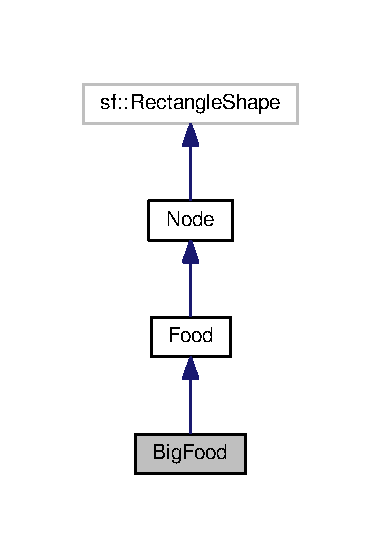
\includegraphics[width=183pt]{classBigFood__inherit__graph}
\end{center}
\end{figure}


Collaboration diagram for Big\+Food\+:\nopagebreak
\begin{figure}[H]
\begin{center}
\leavevmode
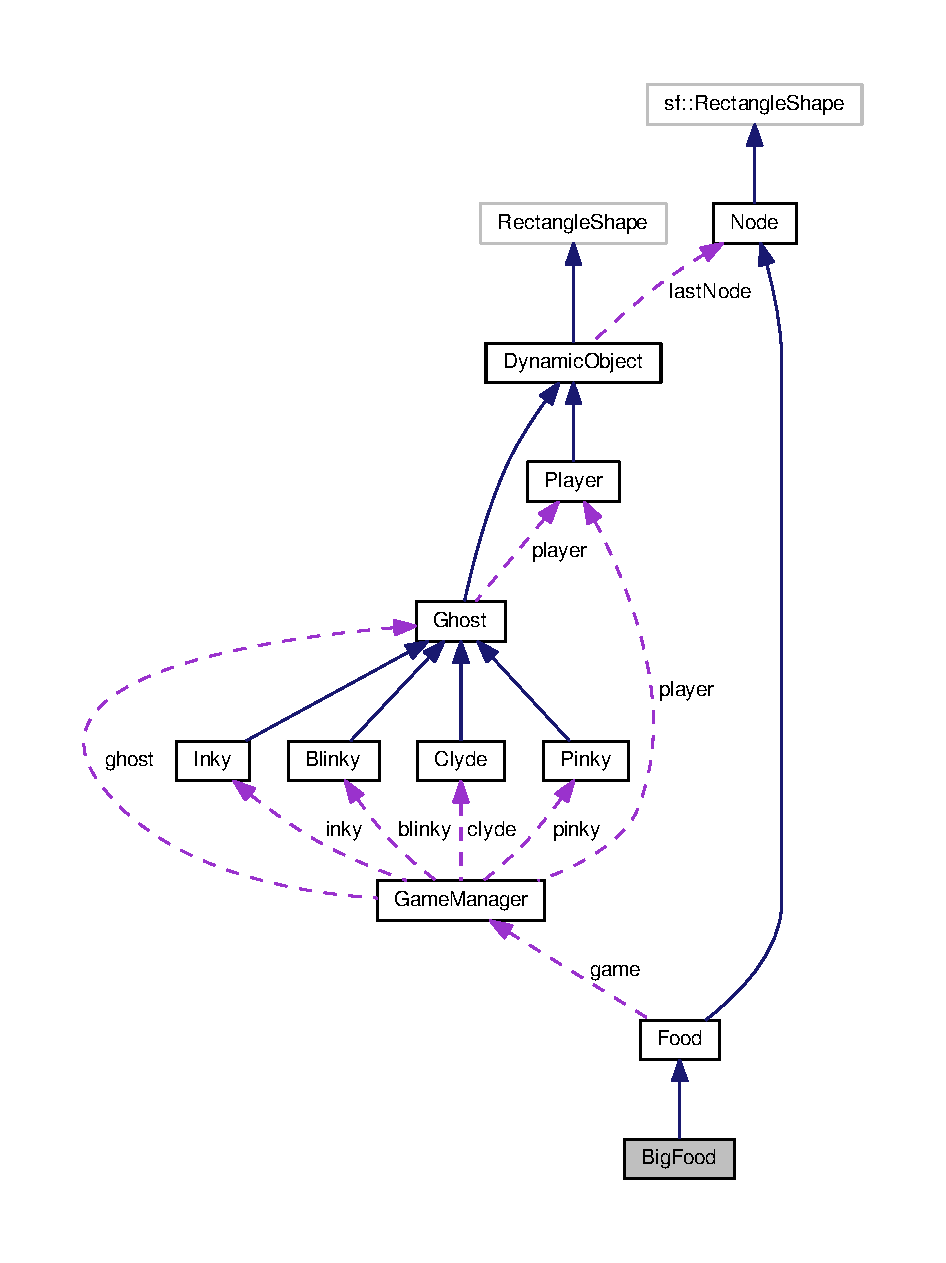
\includegraphics[width=350pt]{classBigFood__coll__graph}
\end{center}
\end{figure}
\subsection*{Public Member Functions}
\begin{DoxyCompactItemize}
\item 
\mbox{\Hypertarget{classBigFood_ae90fad18345d1472c6c10dad2bda4dc4}\label{classBigFood_ae90fad18345d1472c6c10dad2bda4dc4}} 
{\bfseries Big\+Food} (sf\+::\+Vector2f vector, bool u, bool d, bool l, bool r)
\item 
void \hyperlink{classBigFood_ac463d12e08fe29b7414520c50856b450}{visit} ()
\item 
\mbox{\Hypertarget{classBigFood_acc693365e1ae8051b797c6954a2e4e37}\label{classBigFood_acc693365e1ae8051b797c6954a2e4e37}} 
void \hyperlink{classBigFood_acc693365e1ae8051b797c6954a2e4e37}{reset} ()
\begin{DoxyCompactList}\small\item\em Ustawia jedzenie jako niezjedzone. \end{DoxyCompactList}\end{DoxyCompactItemize}
\subsection*{Additional Inherited Members}


\subsection{Detailed Description}
Reprezentuje grube jedzenie, przeznaczone do zjedzenia przez gracza. 

\subsection{Member Function Documentation}
\mbox{\Hypertarget{classBigFood_ac463d12e08fe29b7414520c50856b450}\label{classBigFood_ac463d12e08fe29b7414520c50856b450}} 
\index{Big\+Food@{Big\+Food}!visit@{visit}}
\index{visit@{visit}!Big\+Food@{Big\+Food}}
\subsubsection{\texorpdfstring{visit()}{visit()}}
{\footnotesize\ttfamily void Big\+Food\+::visit (\begin{DoxyParamCaption}{ }\end{DoxyParamCaption})\hspace{0.3cm}{\ttfamily [virtual]}}

Metoda powoduje ustawienie duszków w tryb ucieczki i ustawia kierunek ich ruchu na przeciwny. Obiekt przechodzi w tryb \textquotesingle{}zjedzony\textquotesingle{}. Dodaje 40 do licznika punktów gracza. 

Reimplemented from \hyperlink{classNode_a7cb557af2f8c31fa43fc4c75134750e8}{Node}.



The documentation for this class was generated from the following files\+:\begin{DoxyCompactItemize}
\item 
Engine/Big\+Food.\+h\item 
Engine/Big\+Food.\+cpp\end{DoxyCompactItemize}

\hypertarget{classBlinky}{}\section{Blinky Class Reference}
\label{classBlinky}\index{Blinky@{Blinky}}


Jeden z duszków.  




{\ttfamily \#include $<$Blinky.\+h$>$}



Inheritance diagram for Blinky\+:\nopagebreak
\begin{figure}[H]
\begin{center}
\leavevmode
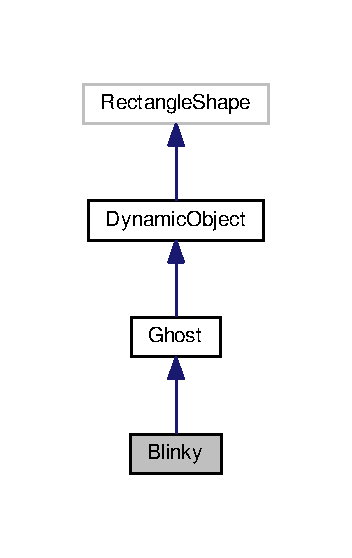
\includegraphics[width=169pt]{classBlinky__inherit__graph}
\end{center}
\end{figure}


Collaboration diagram for Blinky\+:\nopagebreak
\begin{figure}[H]
\begin{center}
\leavevmode
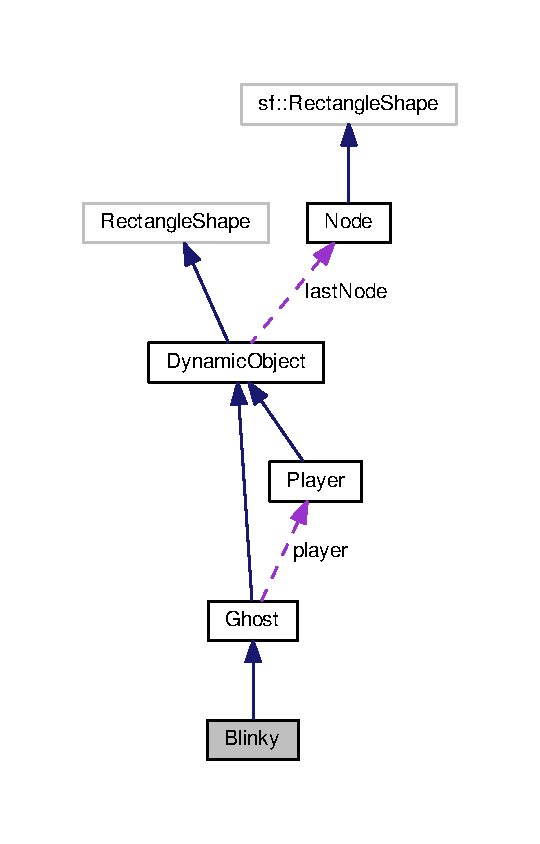
\includegraphics[width=259pt]{classBlinky__coll__graph}
\end{center}
\end{figure}
\subsection*{Public Member Functions}
\begin{DoxyCompactItemize}
\item 
\mbox{\Hypertarget{classBlinky_a1dc22a209b4074b5141e472a16479d68}\label{classBlinky_a1dc22a209b4074b5141e472a16479d68}} 
{\bfseries Blinky} (const sf\+::\+Vector2f \&vector, std\+::vector$<$ \hyperlink{classNode}{Node} $\ast$$>$ \&nodes\+Vector, \hyperlink{classPlayer}{Player} $\ast$player\+Pointer, std\+::vector$<$ \hyperlink{classTunnel}{Tunnel} $\ast$$>$ $\ast$tunnels\+Vector)
\item 
\mbox{\Hypertarget{classBlinky_a801c3ec6c0132364748089029499def9}\label{classBlinky_a801c3ec6c0132364748089029499def9}} 
void \hyperlink{classBlinky_a801c3ec6c0132364748089029499def9}{move} ()
\begin{DoxyCompactList}\small\item\em Wykonuje ruch duszka zgodnie z jego taktyką \end{DoxyCompactList}\end{DoxyCompactItemize}
\subsection*{Additional Inherited Members}


\subsection{Detailed Description}
Jeden z duszków. 

The documentation for this class was generated from the following files\+:\begin{DoxyCompactItemize}
\item 
Engine/Blinky.\+h\item 
Engine/Blinky.\+cpp\end{DoxyCompactItemize}

\hypertarget{classClyde}{}\section{Clyde Class Reference}
\label{classClyde}\index{Clyde@{Clyde}}


Jeden z duszków.  




{\ttfamily \#include $<$Clyde.\+h$>$}



Inheritance diagram for Clyde\+:\nopagebreak
\begin{figure}[H]
\begin{center}
\leavevmode
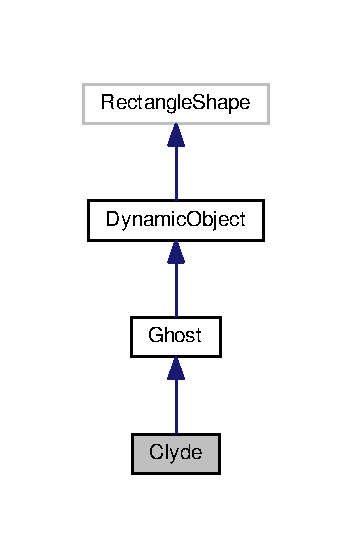
\includegraphics[width=169pt]{classClyde__inherit__graph}
\end{center}
\end{figure}


Collaboration diagram for Clyde\+:\nopagebreak
\begin{figure}[H]
\begin{center}
\leavevmode
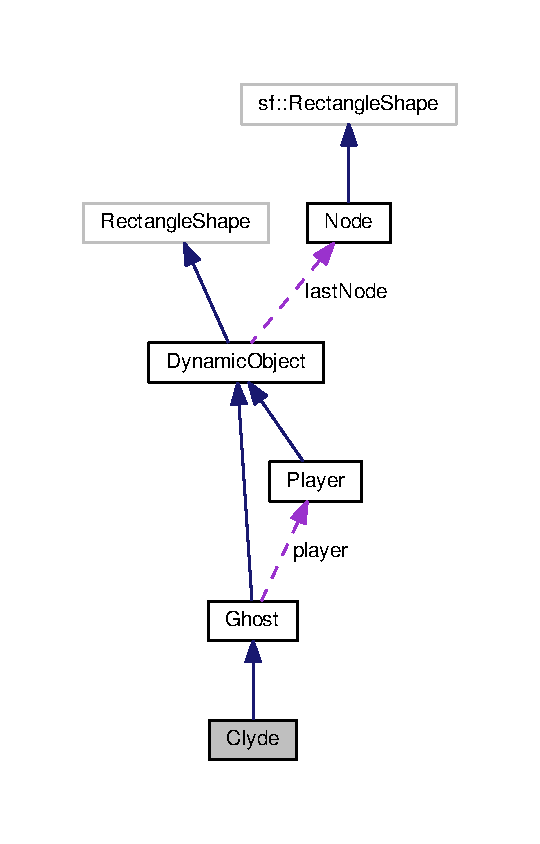
\includegraphics[width=259pt]{classClyde__coll__graph}
\end{center}
\end{figure}
\subsection*{Public Member Functions}
\begin{DoxyCompactItemize}
\item 
\mbox{\Hypertarget{classClyde_a0d8ba4b9949399a78d40d86eef288aa6}\label{classClyde_a0d8ba4b9949399a78d40d86eef288aa6}} 
{\bfseries Clyde} (const sf\+::\+Vector2f \&vector, std\+::vector$<$ \hyperlink{classNode}{Node} $\ast$$>$ \&nodes\+Vector, \hyperlink{classPlayer}{Player} $\ast$player\+Pointer, std\+::vector$<$ \hyperlink{classTunnel}{Tunnel} $\ast$$>$ $\ast$tunnels\+Vector)
\item 
\mbox{\Hypertarget{classClyde_a3ff46c7fcba7062ff7df5cc3ac92ad44}\label{classClyde_a3ff46c7fcba7062ff7df5cc3ac92ad44}} 
void \hyperlink{classClyde_a3ff46c7fcba7062ff7df5cc3ac92ad44}{move} ()
\begin{DoxyCompactList}\small\item\em Wykonuje ruch duszka zgodnie z jego taktyką \end{DoxyCompactList}\end{DoxyCompactItemize}
\subsection*{Additional Inherited Members}


\subsection{Detailed Description}
Jeden z duszków. 

The documentation for this class was generated from the following files\+:\begin{DoxyCompactItemize}
\item 
Engine/Clyde.\+h\item 
Engine/Clyde.\+cpp\end{DoxyCompactItemize}

\hypertarget{classDynamicObject}{}\section{Dynamic\+Object Class Reference}
\label{classDynamicObject}\index{Dynamic\+Object@{Dynamic\+Object}}


Klasa reprezentująca obiekty poruszające się od węzła do węzła.  




{\ttfamily \#include $<$Dynamic\+Object.\+h$>$}



Inheritance diagram for Dynamic\+Object\+:\nopagebreak
\begin{figure}[H]
\begin{center}
\leavevmode
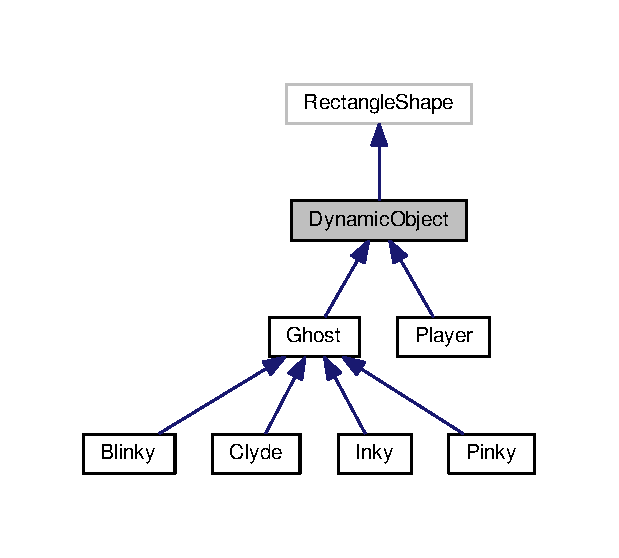
\includegraphics[width=297pt]{classDynamicObject__inherit__graph}
\end{center}
\end{figure}


Collaboration diagram for Dynamic\+Object\+:\nopagebreak
\begin{figure}[H]
\begin{center}
\leavevmode
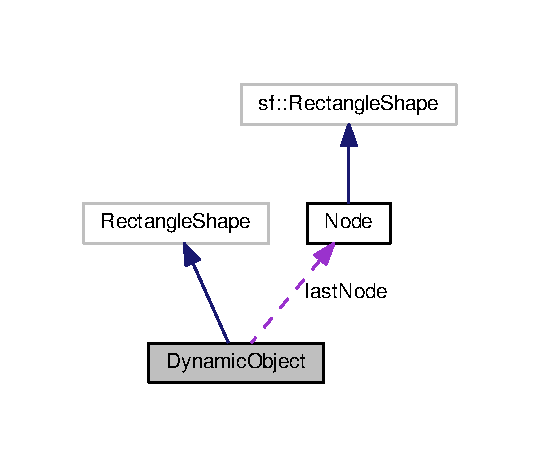
\includegraphics[width=259pt]{classDynamicObject__coll__graph}
\end{center}
\end{figure}
\subsection*{Public Types}
\begin{DoxyCompactItemize}
\item 
\mbox{\Hypertarget{classDynamicObject_a30add874b8507ddd3469e5f9144e8a58}\label{classDynamicObject_a30add874b8507ddd3469e5f9144e8a58}} 
enum {\bfseries Direction} \{ \newline
{\bfseries UP}, 
{\bfseries D\+O\+WN}, 
{\bfseries L\+E\+FT}, 
{\bfseries R\+I\+G\+HT}, 
\newline
{\bfseries N\+O\+NE}
 \}
\end{DoxyCompactItemize}
\subsection*{Public Member Functions}
\begin{DoxyCompactItemize}
\item 
\mbox{\Hypertarget{classDynamicObject_a81829b0b8ee1c8f1b7836522ffa41080}\label{classDynamicObject_a81829b0b8ee1c8f1b7836522ffa41080}} 
void \hyperlink{classDynamicObject_a81829b0b8ee1c8f1b7836522ffa41080}{respawn} ()
\begin{DoxyCompactList}\small\item\em Metoda ustawia obiekt w punkcie określonym przez atrybut spawn\+Point. \end{DoxyCompactList}\end{DoxyCompactItemize}
\subsection*{Public Attributes}
\begin{DoxyCompactItemize}
\item 
\mbox{\Hypertarget{classDynamicObject_ac3934eeb8931556f9dce6d988ab00c6e}\label{classDynamicObject_ac3934eeb8931556f9dce6d988ab00c6e}} 
Direction {\bfseries last\+Wanted\+Direction}
\end{DoxyCompactItemize}
\subsection*{Protected Member Functions}
\begin{DoxyCompactItemize}
\item 
\hyperlink{classNode}{Node} $\ast$ \hyperlink{classDynamicObject_af121dbd6d880bf772494ae251e272693}{is\+In\+Node} ()
\begin{DoxyCompactList}\small\item\em Sprawdza czy obiekt znajduje się w węźle. \end{DoxyCompactList}\item 
\hyperlink{classDynamicObject_a5e007abd09c1a213c913ec0dbf11be7a}{Dynamic\+Object} (const sf\+::\+Vector2f \&vector, std\+::vector$<$ \hyperlink{classNode}{Node} $\ast$$>$ \&nodes\+Vector)
\begin{DoxyCompactList}\small\item\em Inicjalizuje obiekt dynamiczny. \end{DoxyCompactList}\item 
void \hyperlink{classDynamicObject_a9fb1ce835d8c4ffe0a3ffd799067be9a}{move} ()
\begin{DoxyCompactList}\small\item\em Metoda przesuwa obiekt. \end{DoxyCompactList}\item 
\mbox{\Hypertarget{classDynamicObject_aba876e4dabfefa89c00b9926108216dc}\label{classDynamicObject_aba876e4dabfefa89c00b9926108216dc}} 
void \hyperlink{classDynamicObject_aba876e4dabfefa89c00b9926108216dc}{change\+Movement} (const Direction \&direction)
\begin{DoxyCompactList}\small\item\em Metoda ustawia atrybut movement. \end{DoxyCompactList}\end{DoxyCompactItemize}
\subsection*{Protected Attributes}
\begin{DoxyCompactItemize}
\item 
\mbox{\Hypertarget{classDynamicObject_af5b2bd3854bed73057d1e13fd23a138e}\label{classDynamicObject_af5b2bd3854bed73057d1e13fd23a138e}} 
std\+::vector$<$ \hyperlink{classNode}{Node} $\ast$ $>$ \& \hyperlink{classDynamicObject_af5b2bd3854bed73057d1e13fd23a138e}{nodes}
\begin{DoxyCompactList}\small\item\em Zbiór węzłów na mapie. \end{DoxyCompactList}\item 
\mbox{\Hypertarget{classDynamicObject_a97ec96a61e89872abd56017739638ca0}\label{classDynamicObject_a97ec96a61e89872abd56017739638ca0}} 
Direction \hyperlink{classDynamicObject_a97ec96a61e89872abd56017739638ca0}{movement}
\begin{DoxyCompactList}\small\item\em kierunek następnego ruchu obiektu \end{DoxyCompactList}\item 
\mbox{\Hypertarget{classDynamicObject_aa6a2b1fc0fdfae2ea1b6612638dec4af}\label{classDynamicObject_aa6a2b1fc0fdfae2ea1b6612638dec4af}} 
float {\bfseries speed\+Value}
\item 
\mbox{\Hypertarget{classDynamicObject_adeb1429f88acc030da655f902e300eda}\label{classDynamicObject_adeb1429f88acc030da655f902e300eda}} 
sf\+::\+Vector2f {\bfseries speed}
\item 
\mbox{\Hypertarget{classDynamicObject_a777c530472f9ce9d76e3b77c4ce0a8a7}\label{classDynamicObject_a777c530472f9ce9d76e3b77c4ce0a8a7}} 
\hyperlink{classNode}{Node} $\ast$ {\bfseries last\+Node}
\item 
\mbox{\Hypertarget{classDynamicObject_a21a010faebd39dffd380d72398db8521}\label{classDynamicObject_a21a010faebd39dffd380d72398db8521}} 
sf\+::\+Vector2f {\bfseries spawn\+Point}
\end{DoxyCompactItemize}
\subsection*{Friends}
\begin{DoxyCompactItemize}
\item 
\mbox{\Hypertarget{classDynamicObject_a8ec4a0482122250d43ff5a0eecc335c8}\label{classDynamicObject_a8ec4a0482122250d43ff5a0eecc335c8}} 
class {\bfseries Tunnel}
\item 
\mbox{\Hypertarget{classDynamicObject_a140a2a29511147897abbb772733f6c2c}\label{classDynamicObject_a140a2a29511147897abbb772733f6c2c}} 
class {\bfseries Game\+Manager}
\end{DoxyCompactItemize}


\subsection{Detailed Description}
Klasa reprezentująca obiekty poruszające się od węzła do węzła. 

\subsection{Constructor \& Destructor Documentation}
\mbox{\Hypertarget{classDynamicObject_a5e007abd09c1a213c913ec0dbf11be7a}\label{classDynamicObject_a5e007abd09c1a213c913ec0dbf11be7a}} 
\index{Dynamic\+Object@{Dynamic\+Object}!Dynamic\+Object@{Dynamic\+Object}}
\index{Dynamic\+Object@{Dynamic\+Object}!Dynamic\+Object@{Dynamic\+Object}}
\subsubsection{\texorpdfstring{Dynamic\+Object()}{DynamicObject()}}
{\footnotesize\ttfamily Dynamic\+Object\+::\+Dynamic\+Object (\begin{DoxyParamCaption}\item[{const sf\+::\+Vector2f \&}]{vector,  }\item[{std\+::vector$<$ \hyperlink{classNode}{Node} $\ast$$>$ \&}]{nodes\+Vector }\end{DoxyParamCaption})\hspace{0.3cm}{\ttfamily [protected]}}



Inicjalizuje obiekt dynamiczny. 


\begin{DoxyParams}{Parameters}
{\em vector} & określa położenie obiektu \\
\hline
{\em nodes\+Vector} & wektor przechowujący wskaźniki na wszystkie węzły z planszy \\
\hline
\end{DoxyParams}


\subsection{Member Function Documentation}
\mbox{\Hypertarget{classDynamicObject_af121dbd6d880bf772494ae251e272693}\label{classDynamicObject_af121dbd6d880bf772494ae251e272693}} 
\index{Dynamic\+Object@{Dynamic\+Object}!is\+In\+Node@{is\+In\+Node}}
\index{is\+In\+Node@{is\+In\+Node}!Dynamic\+Object@{Dynamic\+Object}}
\subsubsection{\texorpdfstring{is\+In\+Node()}{isInNode()}}
{\footnotesize\ttfamily \hyperlink{classNode}{Node} $\ast$ Dynamic\+Object\+::is\+In\+Node (\begin{DoxyParamCaption}{ }\end{DoxyParamCaption})\hspace{0.3cm}{\ttfamily [protected]}}



Sprawdza czy obiekt znajduje się w węźle. 

Jeśli obiekt znajduje się w węźle, metoda zwraca wskaźnik na ten węzeł. Jeśli obiekt nie znajduje się w węźle, zwracany jest wskaźnik nullptr \mbox{\Hypertarget{classDynamicObject_a9fb1ce835d8c4ffe0a3ffd799067be9a}\label{classDynamicObject_a9fb1ce835d8c4ffe0a3ffd799067be9a}} 
\index{Dynamic\+Object@{Dynamic\+Object}!move@{move}}
\index{move@{move}!Dynamic\+Object@{Dynamic\+Object}}
\subsubsection{\texorpdfstring{move()}{move()}}
{\footnotesize\ttfamily void Dynamic\+Object\+::move (\begin{DoxyParamCaption}{ }\end{DoxyParamCaption})\hspace{0.3cm}{\ttfamily [protected]}}



Metoda przesuwa obiekt. 

Metoda przesuwa obiekt o pewną ilość pikseli określoną przez wartość atrybutu speed\+Value, w kierunku określonym przez wartość atrybutu movement. 

The documentation for this class was generated from the following files\+:\begin{DoxyCompactItemize}
\item 
Engine/Dynamic\+Object.\+h\item 
Engine/Dynamic\+Object.\+cpp\end{DoxyCompactItemize}

\hypertarget{classFood}{}\section{Food Class Reference}
\label{classFood}\index{Food@{Food}}


Reprezentuje węzły na mapie, które po odwiedzeniu przez gracza zostają \textquotesingle{}zjedzone\textquotesingle{}.  




{\ttfamily \#include $<$Food.\+h$>$}



Inheritance diagram for Food\+:\nopagebreak
\begin{figure}[H]
\begin{center}
\leavevmode
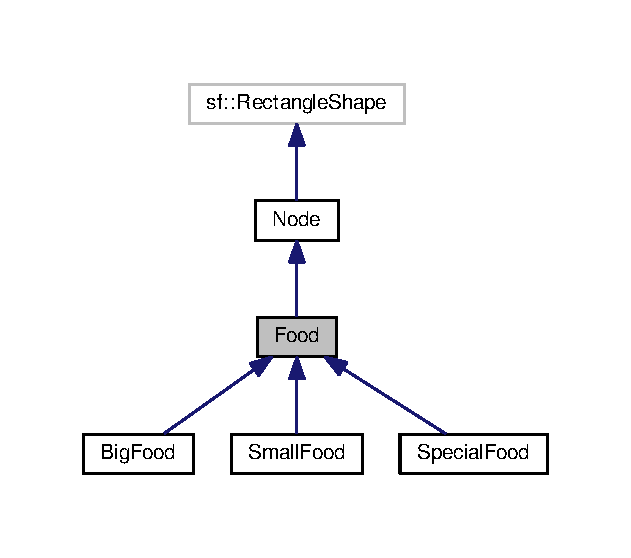
\includegraphics[width=303pt]{classFood__inherit__graph}
\end{center}
\end{figure}


Collaboration diagram for Food\+:\nopagebreak
\begin{figure}[H]
\begin{center}
\leavevmode
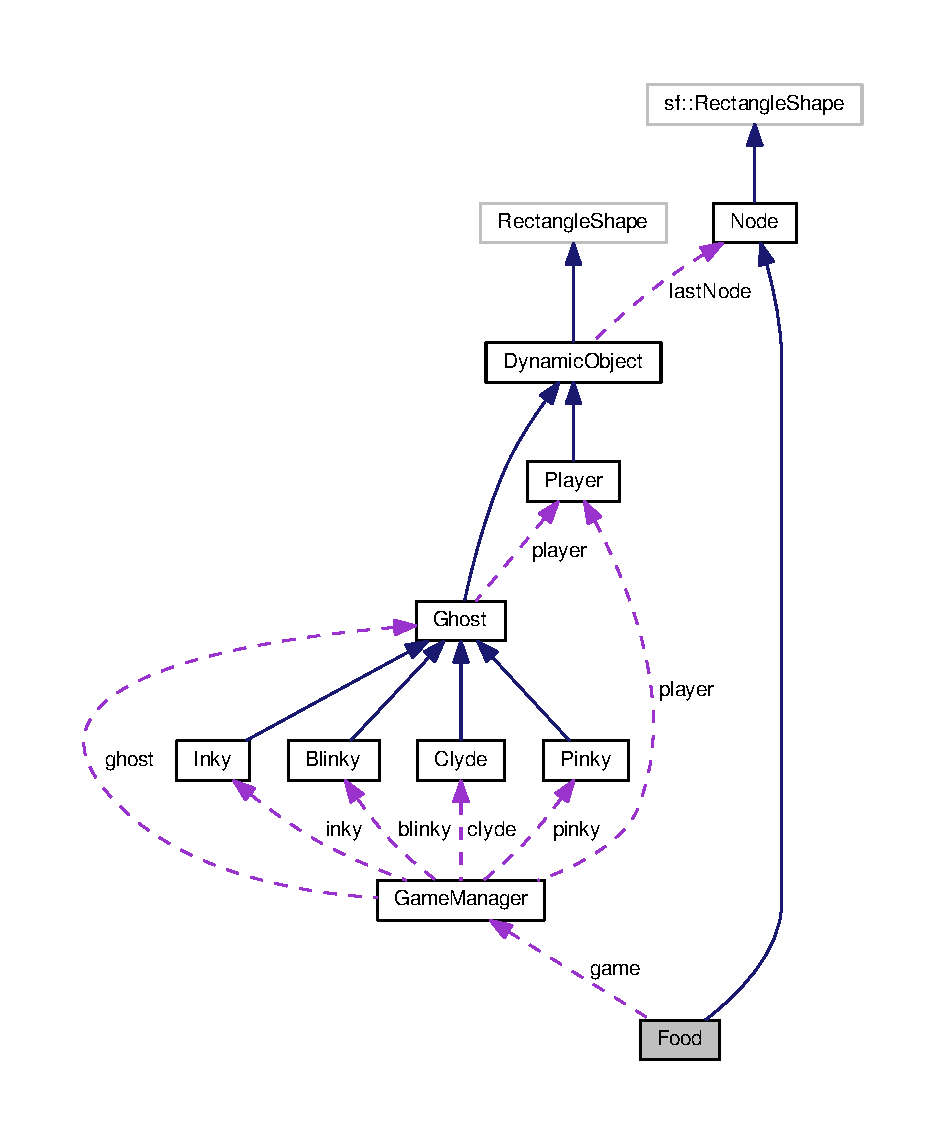
\includegraphics[width=350pt]{classFood__coll__graph}
\end{center}
\end{figure}
\subsection*{Public Member Functions}
\begin{DoxyCompactItemize}
\item 
\mbox{\Hypertarget{classFood_aae0f694b088560c8d826c60911ab2b16}\label{classFood_aae0f694b088560c8d826c60911ab2b16}} 
{\bfseries Food} (sf\+::\+Vector2f vector, bool u, bool d, bool l, bool r)
\end{DoxyCompactItemize}
\subsection*{Public Attributes}
\begin{DoxyCompactItemize}
\item 
\mbox{\Hypertarget{classFood_a2856658914904d30e7276d8a6e382c52}\label{classFood_a2856658914904d30e7276d8a6e382c52}} 
\hyperlink{classGameManager}{Game\+Manager} $\ast$ {\bfseries game}
\end{DoxyCompactItemize}
\subsection*{Protected Attributes}
\begin{DoxyCompactItemize}
\item 
\mbox{\Hypertarget{classFood_a23c6b5d2c4106865a631ef0c9381e36d}\label{classFood_a23c6b5d2c4106865a631ef0c9381e36d}} 
bool {\bfseries is\+Eaten}
\end{DoxyCompactItemize}


\subsection{Detailed Description}
Reprezentuje węzły na mapie, które po odwiedzeniu przez gracza zostają \textquotesingle{}zjedzone\textquotesingle{}. 

The documentation for this class was generated from the following files\+:\begin{DoxyCompactItemize}
\item 
Engine/Food.\+h\item 
Engine/Food.\+cpp\end{DoxyCompactItemize}

\hypertarget{classGameManager}{}\section{Game\+Manager Class Reference}
\label{classGameManager}\index{Game\+Manager@{Game\+Manager}}


Klasa odpowiadająca za sterowanie rozgrywką  




{\ttfamily \#include $<$Game\+Manager.\+h$>$}



Collaboration diagram for Game\+Manager\+:\nopagebreak
\begin{figure}[H]
\begin{center}
\leavevmode
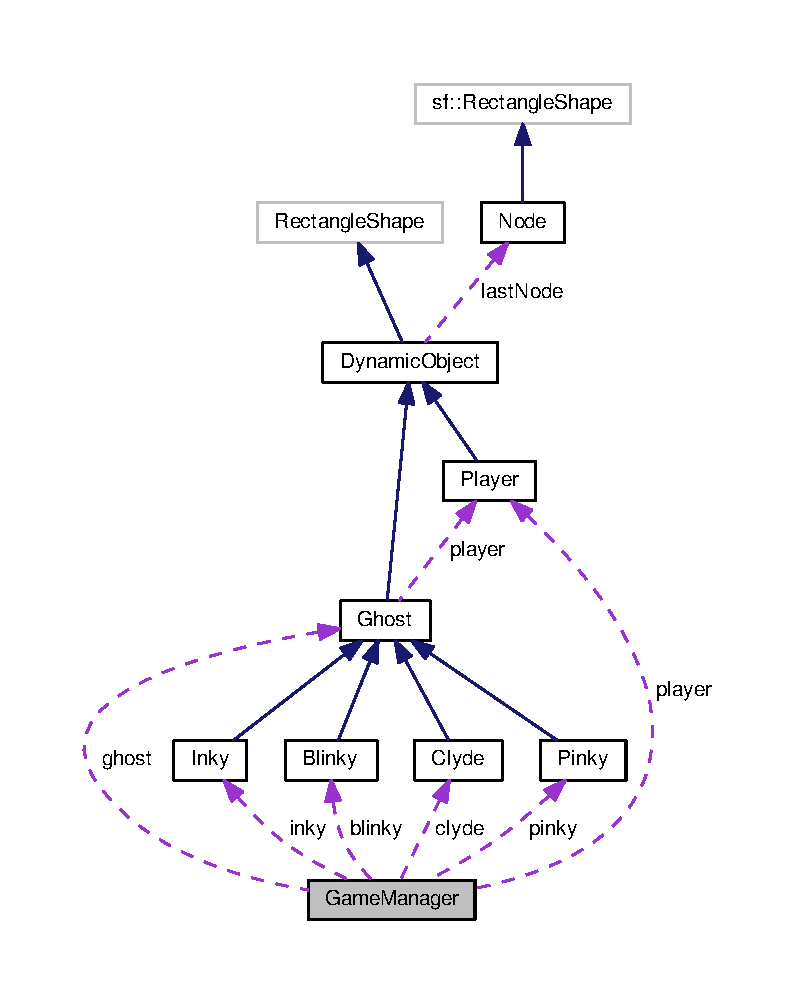
\includegraphics[width=350pt]{classGameManager__coll__graph}
\end{center}
\end{figure}
\subsection*{Public Types}
\begin{DoxyCompactItemize}
\item 
\mbox{\Hypertarget{classGameManager_a809dec58b5681fc1ebcc22eb428a914c}\label{classGameManager_a809dec58b5681fc1ebcc22eb428a914c}} 
enum {\bfseries Game\+State} \{ \newline
{\bfseries B\+E\+F\+O\+R\+E\+R\+O\+U\+ND}, 
{\bfseries R\+A\+N\+D\+OM}, 
{\bfseries H\+U\+NT}, 
{\bfseries E\+S\+C\+A\+PE}, 
\newline
{\bfseries E\+N\+D\+I\+NG}, 
{\bfseries L\+O\+ST}, 
{\bfseries W\+ON}, 
{\bfseries L\+I\+F\+E\+L\+O\+ST}
 \}
\end{DoxyCompactItemize}
\subsection*{Public Member Functions}
\begin{DoxyCompactItemize}
\item 
\hyperlink{classGhost}{Ghost} $\ast$ \hyperlink{classGameManager_affd9b70b3b26c7e6cf09a5a503f87bbf}{is\+Player\+Ghost\+Collision} ()
\begin{DoxyCompactList}\small\item\em Sprawdza czy wystąpiła kolizja gracza z duszkiem. \end{DoxyCompactList}\item 
\mbox{\Hypertarget{classGameManager_af3f088e51e9a9e13d107398bf9591c77}\label{classGameManager_af3f088e51e9a9e13d107398bf9591c77}} 
void \hyperlink{classGameManager_af3f088e51e9a9e13d107398bf9591c77}{action} ()
\begin{DoxyCompactList}\small\item\em Metoda wykonuje kolejną \textquotesingle{}klatkę\textquotesingle{} gry. \end{DoxyCompactList}\item 
\mbox{\Hypertarget{classGameManager_a3aa21d52d6ea7254668136e22c7ea7b6}\label{classGameManager_a3aa21d52d6ea7254668136e22c7ea7b6}} 
void \hyperlink{classGameManager_a3aa21d52d6ea7254668136e22c7ea7b6}{start\+Round} ()
\begin{DoxyCompactList}\small\item\em Metoda tworzy nową rundę gry. \end{DoxyCompactList}\item 
\mbox{\Hypertarget{classGameManager_a94ee1406eebe7612994c73523e388843}\label{classGameManager_a94ee1406eebe7612994c73523e388843}} 
void \hyperlink{classGameManager_a94ee1406eebe7612994c73523e388843}{start\+Random} ()
\begin{DoxyCompactList}\small\item\em Włącza losowy tryb poruszania się duszków. \end{DoxyCompactList}\item 
\mbox{\Hypertarget{classGameManager_a4fad06c8b674c0a8a633cc9cb5efccf5}\label{classGameManager_a4fad06c8b674c0a8a633cc9cb5efccf5}} 
void \hyperlink{classGameManager_a4fad06c8b674c0a8a633cc9cb5efccf5}{start\+Hunt} ()
\begin{DoxyCompactList}\small\item\em Włącza tryb gonitwy. \end{DoxyCompactList}\item 
\mbox{\Hypertarget{classGameManager_a28be7667c0df647cd801b1a01831a849}\label{classGameManager_a28be7667c0df647cd801b1a01831a849}} 
void \hyperlink{classGameManager_a28be7667c0df647cd801b1a01831a849}{start\+Escape} ()
\begin{DoxyCompactList}\small\item\em Włącza tryb ucieczki duszków. \end{DoxyCompactList}\item 
void \hyperlink{classGameManager_a68f66efe17738b9773ce193f032287eb}{start\+Ending} ()
\begin{DoxyCompactList}\small\item\em Włącza tryb końcowy. \end{DoxyCompactList}\item 
\mbox{\Hypertarget{classGameManager_ab7d33de52cc8be9fb9f643a48c11d3b2}\label{classGameManager_ab7d33de52cc8be9fb9f643a48c11d3b2}} 
void \hyperlink{classGameManager_ab7d33de52cc8be9fb9f643a48c11d3b2}{move\+Ghosts} ()
\begin{DoxyCompactList}\small\item\em Metoda powoduje wykonanie swoich ruchów przez duszki. \end{DoxyCompactList}\item 
\mbox{\Hypertarget{classGameManager_ac8492e9ab2b4d660b8ca43fc27259b7e}\label{classGameManager_ac8492e9ab2b4d660b8ca43fc27259b7e}} 
void \hyperlink{classGameManager_ac8492e9ab2b4d660b8ca43fc27259b7e}{reset\+Positions} ()
\begin{DoxyCompactList}\small\item\em Metoda ustawia gracza w pozycje startową, duszki przenosi do klatki. \end{DoxyCompactList}\item 
\mbox{\Hypertarget{classGameManager_a132fab941b740b70c6a7534b25109fbc}\label{classGameManager_a132fab941b740b70c6a7534b25109fbc}} 
void \hyperlink{classGameManager_a132fab941b740b70c6a7534b25109fbc}{reset\+Foods} ()
\begin{DoxyCompactList}\small\item\em Ustawia jedzenie na całej mapie jako niezjedzone. \end{DoxyCompactList}\item 
\mbox{\Hypertarget{classGameManager_a9085b8b46d54303a3111ba38a76f5db5}\label{classGameManager_a9085b8b46d54303a3111ba38a76f5db5}} 
void \hyperlink{classGameManager_a9085b8b46d54303a3111ba38a76f5db5}{reset} ()
\begin{DoxyCompactList}\small\item\em Resetuje cała rozgrywke ( Po porażce gracza ) \end{DoxyCompactList}\end{DoxyCompactItemize}
\subsection*{Public Attributes}
\begin{DoxyCompactItemize}
\item 
\mbox{\Hypertarget{classGameManager_a62299218660ab4144e99485cfdbb4ab3}\label{classGameManager_a62299218660ab4144e99485cfdbb4ab3}} 
unsigned int {\bfseries level}
\item 
\mbox{\Hypertarget{classGameManager_a3d16b7d34c5382f8073bd53a408f2f86}\label{classGameManager_a3d16b7d34c5382f8073bd53a408f2f86}} 
size\+\_\+t {\bfseries points}
\item 
\mbox{\Hypertarget{classGameManager_accc7ea8bcd2eb3f4deba90c257f6077d}\label{classGameManager_accc7ea8bcd2eb3f4deba90c257f6077d}} 
unsigned int {\bfseries lifes}
\item 
\mbox{\Hypertarget{classGameManager_a76367d39b4b431d23c41adfdc788cdd8}\label{classGameManager_a76367d39b4b431d23c41adfdc788cdd8}} 
unsigned int {\bfseries food\+Num}
\item 
\mbox{\Hypertarget{classGameManager_a9578c605b39ae7219e5d609ec8ad3052}\label{classGameManager_a9578c605b39ae7219e5d609ec8ad3052}} 
unsigned int {\bfseries food\+Left}
\item 
\mbox{\Hypertarget{classGameManager_a54960067ed2ad301cd5a8de9aa1b9157}\label{classGameManager_a54960067ed2ad301cd5a8de9aa1b9157}} 
Game\+State {\bfseries state}
\item 
\mbox{\Hypertarget{classGameManager_a796fe777a7517619303e5ba6f0b2431d}\label{classGameManager_a796fe777a7517619303e5ba6f0b2431d}} 
std\+::vector$<$ \hyperlink{classNode}{Node} $\ast$ $>$ {\bfseries nodes}
\item 
\mbox{\Hypertarget{classGameManager_ae6f56a3dc9659110af486af0509ef47e}\label{classGameManager_ae6f56a3dc9659110af486af0509ef47e}} 
std\+::vector$<$ \hyperlink{classSmallFood}{Small\+Food} $\ast$ $>$ {\bfseries small\+Foods}
\item 
\mbox{\Hypertarget{classGameManager_a5147ed76e3a9f8879da5582b54a0ce14}\label{classGameManager_a5147ed76e3a9f8879da5582b54a0ce14}} 
std\+::vector$<$ \hyperlink{classBigFood}{Big\+Food} $\ast$ $>$ {\bfseries big\+Foods}
\item 
\mbox{\Hypertarget{classGameManager_a86b63ff049086d58aa6de0fcd36a0901}\label{classGameManager_a86b63ff049086d58aa6de0fcd36a0901}} 
std\+::vector$<$ \hyperlink{classSpecialFood}{Special\+Food} $\ast$ $>$ {\bfseries special\+Foods}
\item 
\mbox{\Hypertarget{classGameManager_a379cdc5750510e24f5d33abbccd35636}\label{classGameManager_a379cdc5750510e24f5d33abbccd35636}} 
std\+::vector$<$ \hyperlink{classTunnel}{Tunnel} $\ast$ $>$ {\bfseries tunnels}
\item 
\mbox{\Hypertarget{classGameManager_aaf80eea84a37e092f0be3ae6b53dec66}\label{classGameManager_aaf80eea84a37e092f0be3ae6b53dec66}} 
std\+::vector$<$ \hyperlink{classDynamicObject}{Dynamic\+Object} $\ast$ $>$ {\bfseries dynamic\+Objects}
\item 
\mbox{\Hypertarget{classGameManager_af55ae7a2f5c054e6918c283b859de043}\label{classGameManager_af55ae7a2f5c054e6918c283b859de043}} 
std\+::vector$<$ \hyperlink{classGhost}{Ghost} $\ast$ $>$ {\bfseries ghosts}
\item 
\mbox{\Hypertarget{classGameManager_a22f47dea61789d0a10d9967d9084c5d9}\label{classGameManager_a22f47dea61789d0a10d9967d9084c5d9}} 
\hyperlink{classPlayer}{Player} $\ast$ {\bfseries player}
\item 
\mbox{\Hypertarget{classGameManager_a5be78cecbb0c1c0d9b9b114c2dc35d9e}\label{classGameManager_a5be78cecbb0c1c0d9b9b114c2dc35d9e}} 
\hyperlink{classGhost}{Ghost} $\ast$ {\bfseries ghost}
\item 
\mbox{\Hypertarget{classGameManager_a3ff92d6577398553ebd92aeb3ec69c02}\label{classGameManager_a3ff92d6577398553ebd92aeb3ec69c02}} 
\hyperlink{classBlinky}{Blinky} $\ast$ {\bfseries blinky}
\item 
\mbox{\Hypertarget{classGameManager_a2d0c23c7fd47e66e5b0a4ea475d2d62b}\label{classGameManager_a2d0c23c7fd47e66e5b0a4ea475d2d62b}} 
\hyperlink{classInky}{Inky} $\ast$ {\bfseries inky}
\item 
\mbox{\Hypertarget{classGameManager_a581acffc20707de7d41e804917e7593c}\label{classGameManager_a581acffc20707de7d41e804917e7593c}} 
\hyperlink{classPinky}{Pinky} $\ast$ {\bfseries pinky}
\item 
\mbox{\Hypertarget{classGameManager_a1d764f4acb67f7a5b38046321bf8ce03}\label{classGameManager_a1d764f4acb67f7a5b38046321bf8ce03}} 
\hyperlink{classClyde}{Clyde} $\ast$ {\bfseries clyde}
\item 
\mbox{\Hypertarget{classGameManager_a193319c20f58c05b219e95b6374faa2a}\label{classGameManager_a193319c20f58c05b219e95b6374faa2a}} 
bool {\bfseries is\+Start\+Wanted}
\item 
\mbox{\Hypertarget{classGameManager_ae8995792fcb8e8119f1b02230122fb1c}\label{classGameManager_ae8995792fcb8e8119f1b02230122fb1c}} 
size\+\_\+t {\bfseries state\+Timer}
\item 
\mbox{\Hypertarget{classGameManager_acc72348281472430c80ffd848684ce12}\label{classGameManager_acc72348281472430c80ffd848684ce12}} 
size\+\_\+t {\bfseries in\+Cage\+Time}
\item 
\mbox{\Hypertarget{classGameManager_abf0b652a4e156ec223972c7bf6c1eb15}\label{classGameManager_abf0b652a4e156ec223972c7bf6c1eb15}} 
size\+\_\+t {\bfseries random\+Time}
\item 
\mbox{\Hypertarget{classGameManager_a8130420b803aec3db667810ee68b1ef0}\label{classGameManager_a8130420b803aec3db667810ee68b1ef0}} 
size\+\_\+t {\bfseries hunt\+Time}
\item 
\mbox{\Hypertarget{classGameManager_a64ed2adecf7732b25fd0dfe0105f8f22}\label{classGameManager_a64ed2adecf7732b25fd0dfe0105f8f22}} 
size\+\_\+t {\bfseries escape\+Time}
\end{DoxyCompactItemize}


\subsection{Detailed Description}
Klasa odpowiadająca za sterowanie rozgrywką 

\subsection{Member Function Documentation}
\mbox{\Hypertarget{classGameManager_affd9b70b3b26c7e6cf09a5a503f87bbf}\label{classGameManager_affd9b70b3b26c7e6cf09a5a503f87bbf}} 
\index{Game\+Manager@{Game\+Manager}!is\+Player\+Ghost\+Collision@{is\+Player\+Ghost\+Collision}}
\index{is\+Player\+Ghost\+Collision@{is\+Player\+Ghost\+Collision}!Game\+Manager@{Game\+Manager}}
\subsubsection{\texorpdfstring{is\+Player\+Ghost\+Collision()}{isPlayerGhostCollision()}}
{\footnotesize\ttfamily \hyperlink{classGhost}{Ghost} $\ast$ Game\+Manager\+::is\+Player\+Ghost\+Collision (\begin{DoxyParamCaption}{ }\end{DoxyParamCaption})}



Sprawdza czy wystąpiła kolizja gracza z duszkiem. 

Jeśli kolizja wystąpiła, zwracany jest wskaźnik na duszka z którym wystąpiła kolizja. Jeśli nie, zwracany jest wskaźnik nullptr. \mbox{\Hypertarget{classGameManager_a68f66efe17738b9773ce193f032287eb}\label{classGameManager_a68f66efe17738b9773ce193f032287eb}} 
\index{Game\+Manager@{Game\+Manager}!start\+Ending@{start\+Ending}}
\index{start\+Ending@{start\+Ending}!Game\+Manager@{Game\+Manager}}
\subsubsection{\texorpdfstring{start\+Ending()}{startEnding()}}
{\footnotesize\ttfamily void Game\+Manager\+::start\+Ending (\begin{DoxyParamCaption}{ }\end{DoxyParamCaption})}



Włącza tryb końcowy. 

Jest to tryb włączany gdy na planszy zostanie mała ilość jedzenia 

The documentation for this class was generated from the following files\+:\begin{DoxyCompactItemize}
\item 
Engine/Game\+Manager.\+h\item 
Engine/Game\+Manager.\+cpp\end{DoxyCompactItemize}

\hypertarget{classGhost}{}\section{Ghost Class Reference}
\label{classGhost}\index{Ghost@{Ghost}}


Reprezentuje duszka poruszającego się w tunelach.  




{\ttfamily \#include $<$Ghost.\+h$>$}



Inheritance diagram for Ghost\+:\nopagebreak
\begin{figure}[H]
\begin{center}
\leavevmode
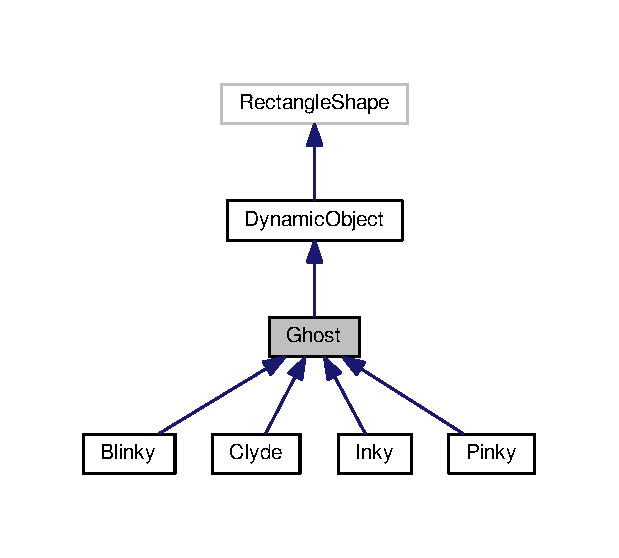
\includegraphics[width=297pt]{classGhost__inherit__graph}
\end{center}
\end{figure}


Collaboration diagram for Ghost\+:\nopagebreak
\begin{figure}[H]
\begin{center}
\leavevmode
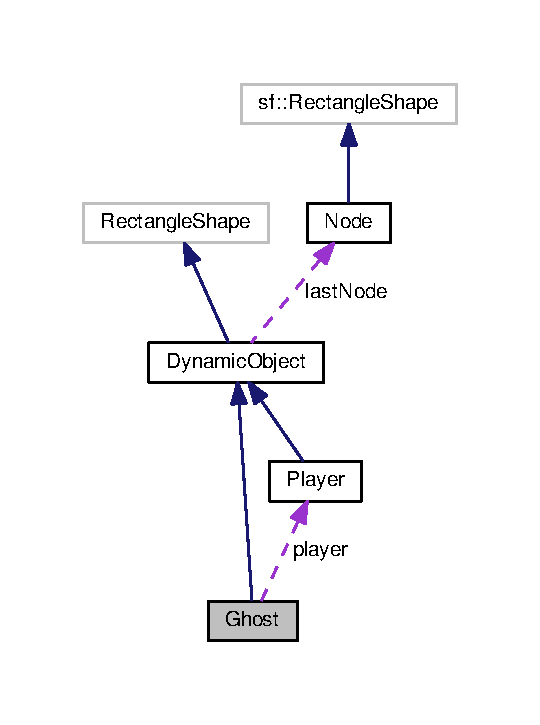
\includegraphics[width=259pt]{classGhost__coll__graph}
\end{center}
\end{figure}
\subsection*{Public Types}
\begin{DoxyCompactItemize}
\item 
\mbox{\Hypertarget{classGhost_af712fc09f900832a0225928c4556234d}\label{classGhost_af712fc09f900832a0225928c4556234d}} 
enum {\bfseries State} \{ {\bfseries R\+A\+N\+D\+OM}, 
{\bfseries H\+U\+NT}, 
{\bfseries E\+S\+C\+A\+PE}
 \}
\end{DoxyCompactItemize}
\subsection*{Public Member Functions}
\begin{DoxyCompactItemize}
\item 
\mbox{\Hypertarget{classGhost_aef285a078acbcc2aecf274fa7954709f}\label{classGhost_aef285a078acbcc2aecf274fa7954709f}} 
{\bfseries Ghost} (const sf\+::\+Vector2f \&vector, std\+::vector$<$ \hyperlink{classNode}{Node} $\ast$$>$ \&nodes\+Vector, \hyperlink{classPlayer}{Player} $\ast$player\+Pointer, std\+::vector$<$ \hyperlink{classTunnel}{Tunnel} $\ast$$>$ $\ast$tunnels)
\item 
\mbox{\Hypertarget{classGhost_afa1fedf2269c2e37fffc70b534b7fa2d}\label{classGhost_afa1fedf2269c2e37fffc70b534b7fa2d}} 
virtual void \hyperlink{classGhost_afa1fedf2269c2e37fffc70b534b7fa2d}{move} ()
\begin{DoxyCompactList}\small\item\em Wykonuje ruch duszka, sposób wykonania ruchu zależy od atrybutu state oraz typu duszka. \end{DoxyCompactList}\item 
\mbox{\Hypertarget{classGhost_aa08c3d40406bcdd8a61739a50b884b10}\label{classGhost_aa08c3d40406bcdd8a61739a50b884b10}} 
void \hyperlink{classGhost_aa08c3d40406bcdd8a61739a50b884b10}{reverse\+Movement} ()
\begin{DoxyCompactList}\small\item\em Zmienia kierunek ruchu duszka na przeciwny. \end{DoxyCompactList}\item 
\mbox{\Hypertarget{classGhost_a658d65b2041de18e5661582d5b1c334c}\label{classGhost_a658d65b2041de18e5661582d5b1c334c}} 
void \hyperlink{classGhost_a658d65b2041de18e5661582d5b1c334c}{respawn} ()
\begin{DoxyCompactList}\small\item\em Ustwaia duszka w tunelu, w pozycji startowej. \end{DoxyCompactList}\item 
\mbox{\Hypertarget{classGhost_a3b81cc4834e50754a0de2343ec6f0aae}\label{classGhost_a3b81cc4834e50754a0de2343ec6f0aae}} 
void \hyperlink{classGhost_a3b81cc4834e50754a0de2343ec6f0aae}{random\+Move} ()
\begin{DoxyCompactList}\small\item\em Wykonuje ruch duszka w losowy ( oczywiście możliwy ) sposób. \end{DoxyCompactList}\item 
\mbox{\Hypertarget{classGhost_a07c89e08fa1fa5ec574cbc846eb839dc}\label{classGhost_a07c89e08fa1fa5ec574cbc846eb839dc}} 
void \hyperlink{classGhost_a07c89e08fa1fa5ec574cbc846eb839dc}{hunt\+Move\+Like\+Blinky} ()
\begin{DoxyCompactList}\small\item\em Wykonuje ruch duszka zgodnie z taktyka ducha \hyperlink{classBlinky}{Blinky} ( można poczytać na wikipedii ) \end{DoxyCompactList}\item 
\mbox{\Hypertarget{classGhost_a38cc82d7c1c5f1db32d68bbebff8137d}\label{classGhost_a38cc82d7c1c5f1db32d68bbebff8137d}} 
void \hyperlink{classGhost_a38cc82d7c1c5f1db32d68bbebff8137d}{hunt\+Move\+Like\+Pinky} ()
\begin{DoxyCompactList}\small\item\em Wykonuje ruch duszka zgodnie z taktyką ducha \hyperlink{classPinky}{Pinky} ( moźna poczytać na wikipedii ) \end{DoxyCompactList}\item 
\mbox{\Hypertarget{classGhost_a3417f9bbc23adc0ad0ff0db7e62580a2}\label{classGhost_a3417f9bbc23adc0ad0ff0db7e62580a2}} 
void \hyperlink{classGhost_a3417f9bbc23adc0ad0ff0db7e62580a2}{escape\+Move} ()
\begin{DoxyCompactList}\small\item\em Wykonuje ruch w taki sposób by uciekać przed graczem. \end{DoxyCompactList}\item 
\mbox{\Hypertarget{classGhost_aeac8841dffd0f8c1c21669b43c710008}\label{classGhost_aeac8841dffd0f8c1c21669b43c710008}} 
void \hyperlink{classGhost_aeac8841dffd0f8c1c21669b43c710008}{go\+To\+Cage} ()
\begin{DoxyCompactList}\small\item\em Umieszcza gracza w klatce. Wyłącza go z gry. \end{DoxyCompactList}\item 
\mbox{\Hypertarget{classGhost_a14cf85337a797013fd73f506950a8853}\label{classGhost_a14cf85337a797013fd73f506950a8853}} 
int {\bfseries player\+Position} ()
\end{DoxyCompactItemize}
\subsection*{Public Attributes}
\begin{DoxyCompactItemize}
\item 
\mbox{\Hypertarget{classGhost_a6b7e1f6e9e5ef6767d4b80429088c00a}\label{classGhost_a6b7e1f6e9e5ef6767d4b80429088c00a}} 
State {\bfseries state}
\item 
\mbox{\Hypertarget{classGhost_ab4919b308d77f53f5ca29077633ccb8f}\label{classGhost_ab4919b308d77f53f5ca29077633ccb8f}} 
\hyperlink{classPlayer}{Player} $\ast$ {\bfseries player}
\item 
\mbox{\Hypertarget{classGhost_a312091529dd2c63266aa9acf7bc968c8}\label{classGhost_a312091529dd2c63266aa9acf7bc968c8}} 
std\+::vector$<$ \hyperlink{classTunnel}{Tunnel} $\ast$ $>$ $\ast$ {\bfseries tunnels}
\item 
\mbox{\Hypertarget{classGhost_aa63992f9728d0daa362c6e74884f51ec}\label{classGhost_aa63992f9728d0daa362c6e74884f51ec}} 
bool {\bfseries is\+In\+Cage}
\item 
\mbox{\Hypertarget{classGhost_aaa355fe13f96b7665d3218ba82008248}\label{classGhost_aaa355fe13f96b7665d3218ba82008248}} 
size\+\_\+t {\bfseries time\+In\+Cage}
\item 
\mbox{\Hypertarget{classGhost_aca51db20e7a8357ab1d36bfc58873a71}\label{classGhost_aca51db20e7a8357ab1d36bfc58873a71}} 
int {\bfseries randomization}
\item 
\mbox{\Hypertarget{classGhost_a4ab03d6825c037262095c320df35fc6b}\label{classGhost_a4ab03d6825c037262095c320df35fc6b}} 
sf\+::\+Vector2f {\bfseries position\+In\+Cage}
\end{DoxyCompactItemize}
\subsection*{Additional Inherited Members}


\subsection{Detailed Description}
Reprezentuje duszka poruszającego się w tunelach. 

The documentation for this class was generated from the following files\+:\begin{DoxyCompactItemize}
\item 
Engine/Ghost.\+h\item 
Engine/Ghost.\+cpp\end{DoxyCompactItemize}

\hypertarget{classInky}{}\section{Inky Class Reference}
\label{classInky}\index{Inky@{Inky}}


Jeden z duszków.  




{\ttfamily \#include $<$Inky.\+h$>$}



Inheritance diagram for Inky\+:\nopagebreak
\begin{figure}[H]
\begin{center}
\leavevmode
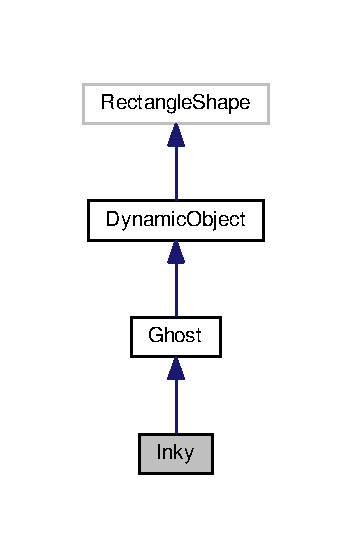
\includegraphics[width=169pt]{classInky__inherit__graph}
\end{center}
\end{figure}


Collaboration diagram for Inky\+:\nopagebreak
\begin{figure}[H]
\begin{center}
\leavevmode
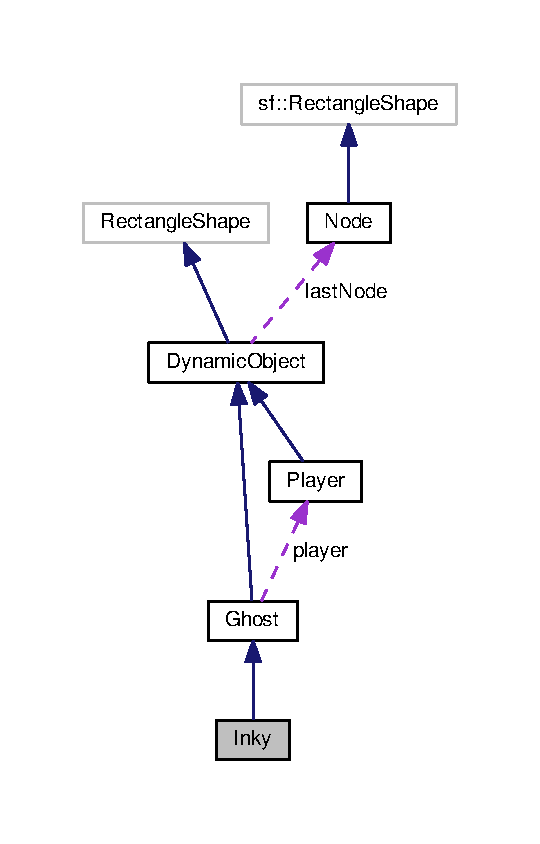
\includegraphics[width=259pt]{classInky__coll__graph}
\end{center}
\end{figure}
\subsection*{Public Member Functions}
\begin{DoxyCompactItemize}
\item 
\mbox{\Hypertarget{classInky_aa961db3b657615d617044c26ecfbd487}\label{classInky_aa961db3b657615d617044c26ecfbd487}} 
{\bfseries Inky} (const sf\+::\+Vector2f \&vector, std\+::vector$<$ \hyperlink{classNode}{Node} $\ast$$>$ \&nodes\+Vector, \hyperlink{classPlayer}{Player} $\ast$player\+Pointer, std\+::vector$<$ \hyperlink{classTunnel}{Tunnel} $\ast$$>$ $\ast$tunnels\+Vector)
\item 
\mbox{\Hypertarget{classInky_a693b31f383ea21c1164d482edb7d868c}\label{classInky_a693b31f383ea21c1164d482edb7d868c}} 
void \hyperlink{classInky_a693b31f383ea21c1164d482edb7d868c}{move} ()
\begin{DoxyCompactList}\small\item\em Wykonuje ruch duszka zgodnie z jego taktyką \end{DoxyCompactList}\end{DoxyCompactItemize}
\subsection*{Additional Inherited Members}


\subsection{Detailed Description}
Jeden z duszków. 

The documentation for this class was generated from the following files\+:\begin{DoxyCompactItemize}
\item 
Engine/Inky.\+h\item 
Engine/Inky.\+cpp\end{DoxyCompactItemize}

\hypertarget{classNode}{}\section{Node Class Reference}
\label{classNode}\index{Node@{Node}}


Reprezentuje węzel. Pewny punkt na mapie.  




{\ttfamily \#include $<$Node.\+h$>$}



Inheritance diagram for Node\+:\nopagebreak
\begin{figure}[H]
\begin{center}
\leavevmode
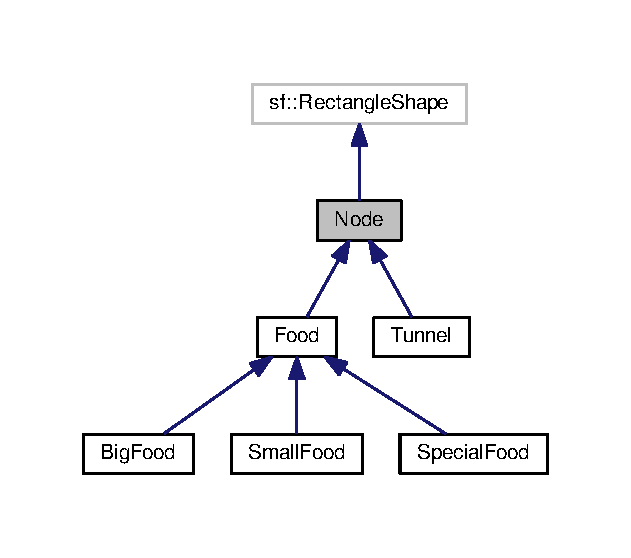
\includegraphics[width=303pt]{classNode__inherit__graph}
\end{center}
\end{figure}


Collaboration diagram for Node\+:\nopagebreak
\begin{figure}[H]
\begin{center}
\leavevmode
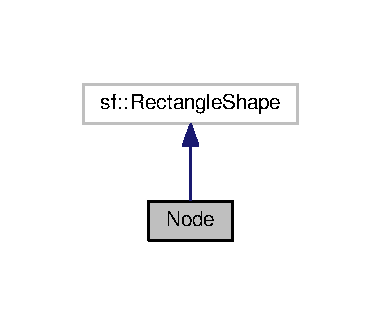
\includegraphics[width=183pt]{classNode__coll__graph}
\end{center}
\end{figure}
\subsection*{Public Member Functions}
\begin{DoxyCompactItemize}
\item 
\hyperlink{classNode_a691046668b01fa3af260a3891c993f99}{Node} (sf\+::\+Vector2f vector, bool u, bool d, bool l, bool r)
\item 
\mbox{\Hypertarget{classNode_a7cb557af2f8c31fa43fc4c75134750e8}\label{classNode_a7cb557af2f8c31fa43fc4c75134750e8}} 
virtual void \hyperlink{classNode_a7cb557af2f8c31fa43fc4c75134750e8}{visit} ()
\begin{DoxyCompactList}\small\item\em Funkcja wywoływana przez obiekty wchodzące do węzła. \end{DoxyCompactList}\item 
\mbox{\Hypertarget{classNode_a3076b2ad2aa24bad4d7989c40ed0c78c}\label{classNode_a3076b2ad2aa24bad4d7989c40ed0c78c}} 
\hyperlink{classNode}{Node} $\ast$ \hyperlink{classNode_a3076b2ad2aa24bad4d7989c40ed0c78c}{get\+Node\+Up} ()
\begin{DoxyCompactList}\small\item\em Zwraca wskaźnik na sąsiadujący węzeł z góry. \end{DoxyCompactList}\item 
\mbox{\Hypertarget{classNode_a9f1fb40744611d9bf3c6bce26b3c6b25}\label{classNode_a9f1fb40744611d9bf3c6bce26b3c6b25}} 
\hyperlink{classNode}{Node} $\ast$ \hyperlink{classNode_a9f1fb40744611d9bf3c6bce26b3c6b25}{get\+Node\+Down} ()
\begin{DoxyCompactList}\small\item\em Zwraca wskaźnik na sąsiadujący węzeł z dołu. \end{DoxyCompactList}\item 
\mbox{\Hypertarget{classNode_a1d337ac51fa169f1d282d97f34caa2e7}\label{classNode_a1d337ac51fa169f1d282d97f34caa2e7}} 
\hyperlink{classNode}{Node} $\ast$ \hyperlink{classNode_a1d337ac51fa169f1d282d97f34caa2e7}{get\+Node\+Left} ()
\begin{DoxyCompactList}\small\item\em Zwraca wskaźnik na sąsiadujący węzeł z lewej. \end{DoxyCompactList}\item 
\mbox{\Hypertarget{classNode_a3a10a1a2f045b29f38d2258e40d06160}\label{classNode_a3a10a1a2f045b29f38d2258e40d06160}} 
\hyperlink{classNode}{Node} $\ast$ \hyperlink{classNode_a3a10a1a2f045b29f38d2258e40d06160}{get\+Node\+Right} ()
\begin{DoxyCompactList}\small\item\em Zwraca wskaźnik na sąsiadujący węzeł z prawej. \end{DoxyCompactList}\end{DoxyCompactItemize}
\subsection*{Public Attributes}
\begin{DoxyCompactItemize}
\item 
\mbox{\Hypertarget{classNode_a27f215e6d295a677f2ad702ca2083001}\label{classNode_a27f215e6d295a677f2ad702ca2083001}} 
const bool {\bfseries up}
\item 
\mbox{\Hypertarget{classNode_a71977171a0abc49390c0c7a7976d4a84}\label{classNode_a71977171a0abc49390c0c7a7976d4a84}} 
const bool {\bfseries down}
\item 
\mbox{\Hypertarget{classNode_a6c681f5bc130c9da117cfc0b79d39403}\label{classNode_a6c681f5bc130c9da117cfc0b79d39403}} 
const bool {\bfseries left}
\item 
\mbox{\Hypertarget{classNode_ae205eb30fb98f214e47c1ca986d0b4d1}\label{classNode_ae205eb30fb98f214e47c1ca986d0b4d1}} 
const bool {\bfseries right}
\end{DoxyCompactItemize}
\subsection*{Friends}
\begin{DoxyCompactItemize}
\item 
\mbox{\Hypertarget{classNode_ab3dcf7a71a5faa0435fdf9db8d28f7f7}\label{classNode_ab3dcf7a71a5faa0435fdf9db8d28f7f7}} 
class {\bfseries Nodes\+Generator}
\end{DoxyCompactItemize}


\subsection{Detailed Description}
Reprezentuje węzel. Pewny punkt na mapie. 

\subsection{Constructor \& Destructor Documentation}
\mbox{\Hypertarget{classNode_a691046668b01fa3af260a3891c993f99}\label{classNode_a691046668b01fa3af260a3891c993f99}} 
\index{Node@{Node}!Node@{Node}}
\index{Node@{Node}!Node@{Node}}
\subsubsection{\texorpdfstring{Node()}{Node()}}
{\footnotesize\ttfamily Node\+::\+Node (\begin{DoxyParamCaption}\item[{sf\+::\+Vector2f}]{vector,  }\item[{bool}]{u,  }\item[{bool}]{d,  }\item[{bool}]{l,  }\item[{bool}]{r }\end{DoxyParamCaption})}


\begin{DoxyParams}{Parameters}
{\em vector} & reprezentuje położenie węzła \\
\hline
{\em u} & posiadanie górnego sąsiada \\
\hline
{\em d} & posiadanie dolnego sąsiada \\
\hline
{\em l} & posiadanie lewego sąsiada \\
\hline
{\em r} & posiadanie prawego sąsiada \\
\hline
\end{DoxyParams}


The documentation for this class was generated from the following files\+:\begin{DoxyCompactItemize}
\item 
Engine/Node.\+h\item 
Engine/Node.\+cpp\end{DoxyCompactItemize}

\hypertarget{classNodesGenerator}{}\section{Nodes\+Generator Class Reference}
\label{classNodesGenerator}\index{Nodes\+Generator@{Nodes\+Generator}}


Generuje mape węzłów ( zwykłe węzły, jedzienie i teleportujący tunel )  




{\ttfamily \#include $<$Nodes\+Generator.\+h$>$}

\subsection*{Public Member Functions}
\begin{DoxyCompactItemize}
\item 
\mbox{\Hypertarget{classNodesGenerator_a8a67eb353d2df91f87ebac5394e799dd}\label{classNodesGenerator_a8a67eb353d2df91f87ebac5394e799dd}} 
{\bfseries Nodes\+Generator} (std\+::vector$<$ \hyperlink{classNode}{Node} $\ast$$>$ \&nodes, std\+::vector$<$ \hyperlink{classSmallFood}{Small\+Food} $\ast$$>$ \&small\+Foods, std\+::vector$<$ \hyperlink{classBigFood}{Big\+Food} $\ast$$>$ \&big\+Foods, std\+::vector$<$ \hyperlink{classSpecialFood}{Special\+Food} $\ast$$>$ \&special\+Foods, std\+::vector$<$ \hyperlink{classTunnel}{Tunnel} $\ast$$>$ \&tunnels, sf\+::\+Vector2f left\+Up\+Corner)
\end{DoxyCompactItemize}


\subsection{Detailed Description}
Generuje mape węzłów ( zwykłe węzły, jedzienie i teleportujący tunel ) 

The documentation for this class was generated from the following files\+:\begin{DoxyCompactItemize}
\item 
Engine/Nodes\+Generator.\+h\item 
Engine/Nodes\+Generator.\+cpp\end{DoxyCompactItemize}

\hypertarget{classPinky}{}\section{Pinky Class Reference}
\label{classPinky}\index{Pinky@{Pinky}}


Jeden z duszków.  




{\ttfamily \#include $<$Pinky.\+h$>$}



Inheritance diagram for Pinky\+:\nopagebreak
\begin{figure}[H]
\begin{center}
\leavevmode
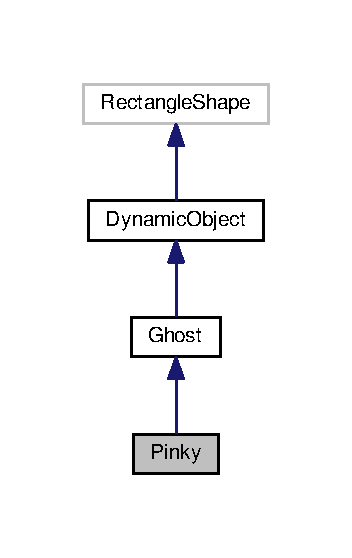
\includegraphics[width=169pt]{classPinky__inherit__graph}
\end{center}
\end{figure}


Collaboration diagram for Pinky\+:\nopagebreak
\begin{figure}[H]
\begin{center}
\leavevmode
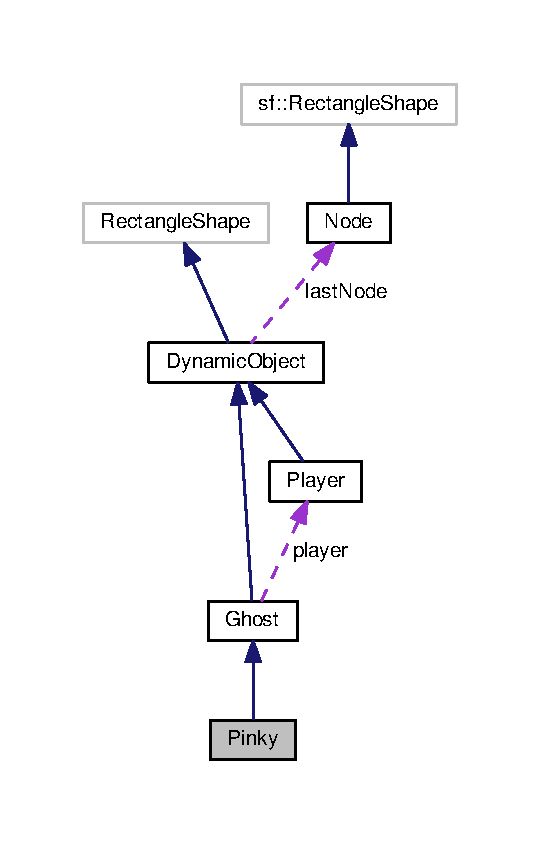
\includegraphics[width=259pt]{classPinky__coll__graph}
\end{center}
\end{figure}
\subsection*{Public Member Functions}
\begin{DoxyCompactItemize}
\item 
\mbox{\Hypertarget{classPinky_a6f64c92d7359c3d7694a9d6e5d73c1a9}\label{classPinky_a6f64c92d7359c3d7694a9d6e5d73c1a9}} 
{\bfseries Pinky} (const sf\+::\+Vector2f \&vector, std\+::vector$<$ \hyperlink{classNode}{Node} $\ast$$>$ \&nodes\+Vector, \hyperlink{classPlayer}{Player} $\ast$player\+Pointer, std\+::vector$<$ \hyperlink{classTunnel}{Tunnel} $\ast$$>$ $\ast$tunnels\+Vector)
\item 
\mbox{\Hypertarget{classPinky_afaa17045a3d876bafecc3f77bbc295ff}\label{classPinky_afaa17045a3d876bafecc3f77bbc295ff}} 
void \hyperlink{classPinky_afaa17045a3d876bafecc3f77bbc295ff}{move} ()
\begin{DoxyCompactList}\small\item\em Wykonuje ruch duszka zgodnie z jego taktyką \end{DoxyCompactList}\end{DoxyCompactItemize}
\subsection*{Additional Inherited Members}


\subsection{Detailed Description}
Jeden z duszków. 

The documentation for this class was generated from the following files\+:\begin{DoxyCompactItemize}
\item 
Engine/Pinky.\+h\item 
Engine/Pinky.\+cpp\end{DoxyCompactItemize}

\hypertarget{classPlayer}{}\section{Player Class Reference}
\label{classPlayer}\index{Player@{Player}}


reprezentuje gracza poruszającego się po mapie  




{\ttfamily \#include $<$Player.\+h$>$}



Inheritance diagram for Player\+:\nopagebreak
\begin{figure}[H]
\begin{center}
\leavevmode
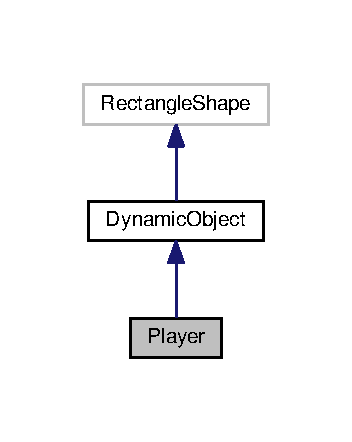
\includegraphics[width=169pt]{classPlayer__inherit__graph}
\end{center}
\end{figure}


Collaboration diagram for Player\+:\nopagebreak
\begin{figure}[H]
\begin{center}
\leavevmode
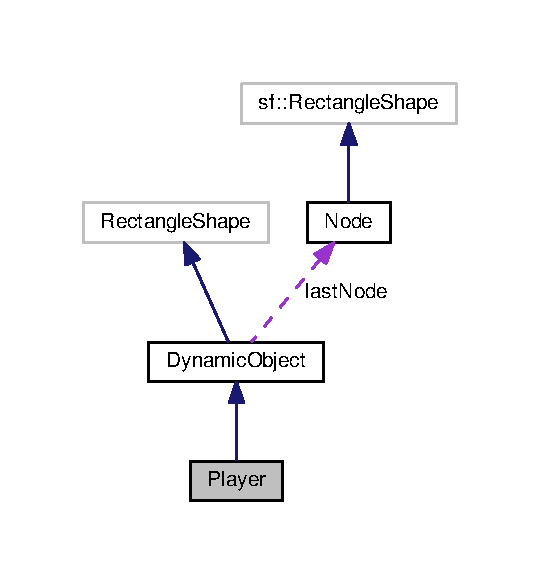
\includegraphics[width=259pt]{classPlayer__coll__graph}
\end{center}
\end{figure}
\subsection*{Public Member Functions}
\begin{DoxyCompactItemize}
\item 
\mbox{\Hypertarget{classPlayer_a6871bb5e4676deda9e7131715590b755}\label{classPlayer_a6871bb5e4676deda9e7131715590b755}} 
{\bfseries Player} (const sf\+::\+Vector2f \&vector, std\+::vector$<$ \hyperlink{classNode}{Node} $\ast$$>$ \&nodes\+Vector)
\item 
void \hyperlink{classPlayer_ae02ee46d8c20dd0697b975f935b09839}{move} ()
\begin{DoxyCompactList}\small\item\em Wykonuje ruch gracza. \end{DoxyCompactList}\end{DoxyCompactItemize}
\subsection*{Friends}
\begin{DoxyCompactItemize}
\item 
\mbox{\Hypertarget{classPlayer_a374118a2c0cb35d1c0fdf7dd8555cda8}\label{classPlayer_a374118a2c0cb35d1c0fdf7dd8555cda8}} 
class {\bfseries Ghost}
\end{DoxyCompactItemize}
\subsection*{Additional Inherited Members}


\subsection{Detailed Description}
reprezentuje gracza poruszającego się po mapie 

\subsection{Member Function Documentation}
\mbox{\Hypertarget{classPlayer_ae02ee46d8c20dd0697b975f935b09839}\label{classPlayer_ae02ee46d8c20dd0697b975f935b09839}} 
\index{Player@{Player}!move@{move}}
\index{move@{move}!Player@{Player}}
\subsubsection{\texorpdfstring{move()}{move()}}
{\footnotesize\ttfamily void Player\+::move (\begin{DoxyParamCaption}{ }\end{DoxyParamCaption})}



Wykonuje ruch gracza. 

Wykonuje ruch gracza w kierunku określonym przez dziedziczony atrybut last\+Wanted\+Direction. Jeśli ruch jest niemożliwy, gracz nie wykonuje ruchu. 

The documentation for this class was generated from the following files\+:\begin{DoxyCompactItemize}
\item 
Engine/Player.\+h\item 
Engine/Player.\+cpp\end{DoxyCompactItemize}

\hypertarget{classSmallFood}{}\section{Small\+Food Class Reference}
\label{classSmallFood}\index{Small\+Food@{Small\+Food}}


Reprezentuje mały obiekt do zjedzenia przez gracza.  




{\ttfamily \#include $<$Small\+Food.\+h$>$}



Inheritance diagram for Small\+Food\+:\nopagebreak
\begin{figure}[H]
\begin{center}
\leavevmode
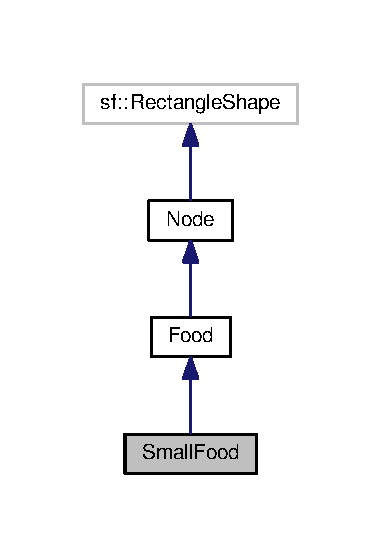
\includegraphics[width=183pt]{classSmallFood__inherit__graph}
\end{center}
\end{figure}


Collaboration diagram for Small\+Food\+:\nopagebreak
\begin{figure}[H]
\begin{center}
\leavevmode
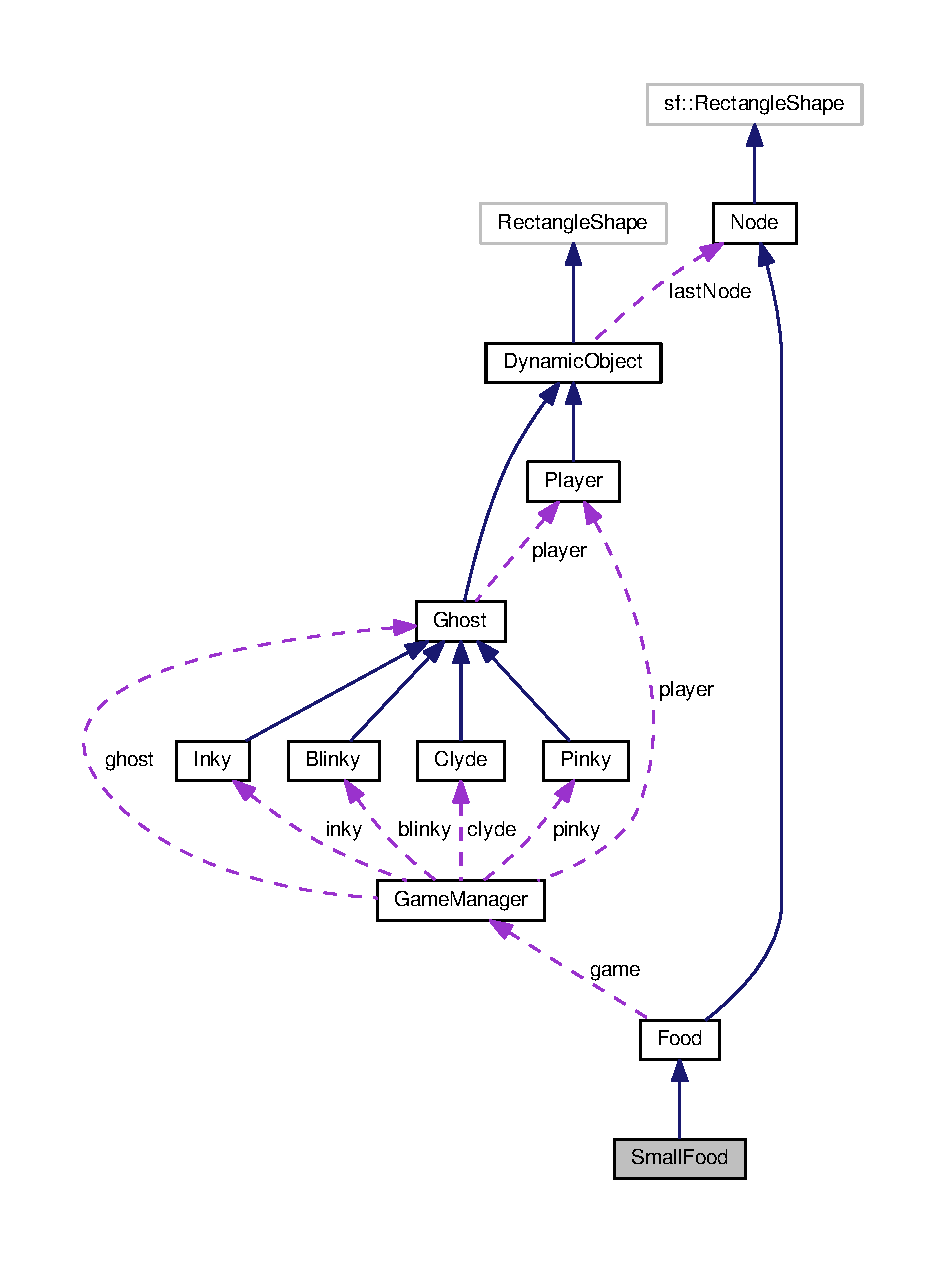
\includegraphics[width=350pt]{classSmallFood__coll__graph}
\end{center}
\end{figure}
\subsection*{Public Member Functions}
\begin{DoxyCompactItemize}
\item 
\mbox{\Hypertarget{classSmallFood_a4d91b2c99fac555ed8c7644ea11a4fe7}\label{classSmallFood_a4d91b2c99fac555ed8c7644ea11a4fe7}} 
{\bfseries Small\+Food} (sf\+::\+Vector2f vector, bool u, bool d, bool l, bool r)
\item 
void \hyperlink{classSmallFood_a4b7a54f8b6c4045dba6c50f117923c01}{visit} ()
\item 
\mbox{\Hypertarget{classSmallFood_a9a2732eae205f0a3c9c17c38d69ff8a4}\label{classSmallFood_a9a2732eae205f0a3c9c17c38d69ff8a4}} 
void \hyperlink{classSmallFood_a9a2732eae205f0a3c9c17c38d69ff8a4}{reset} ()
\begin{DoxyCompactList}\small\item\em Ustawia obiekt jako niezjedzony. \end{DoxyCompactList}\end{DoxyCompactItemize}
\subsection*{Additional Inherited Members}


\subsection{Detailed Description}
Reprezentuje mały obiekt do zjedzenia przez gracza. 

\subsection{Member Function Documentation}
\mbox{\Hypertarget{classSmallFood_a4b7a54f8b6c4045dba6c50f117923c01}\label{classSmallFood_a4b7a54f8b6c4045dba6c50f117923c01}} 
\index{Small\+Food@{Small\+Food}!visit@{visit}}
\index{visit@{visit}!Small\+Food@{Small\+Food}}
\subsubsection{\texorpdfstring{visit()}{visit()}}
{\footnotesize\ttfamily void Small\+Food\+::visit (\begin{DoxyParamCaption}{ }\end{DoxyParamCaption})\hspace{0.3cm}{\ttfamily [virtual]}}

Ustawia obiekt w tryb zjedzony i dodaje 10 do licznika punków gracza. 

Reimplemented from \hyperlink{classNode_a7cb557af2f8c31fa43fc4c75134750e8}{Node}.



The documentation for this class was generated from the following files\+:\begin{DoxyCompactItemize}
\item 
Engine/Small\+Food.\+h\item 
Engine/Small\+Food.\+cpp\end{DoxyCompactItemize}

\hypertarget{classSpecialFood}{}\section{Special\+Food Class Reference}
\label{classSpecialFood}\index{Special\+Food@{Special\+Food}}


T\+O\+DO.  




{\ttfamily \#include $<$Special\+Food.\+h$>$}



Inheritance diagram for Special\+Food\+:\nopagebreak
\begin{figure}[H]
\begin{center}
\leavevmode
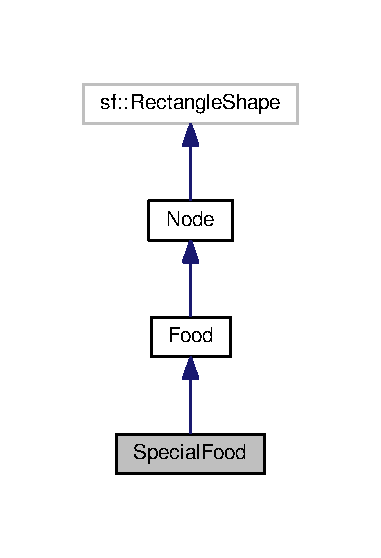
\includegraphics[width=183pt]{classSpecialFood__inherit__graph}
\end{center}
\end{figure}


Collaboration diagram for Special\+Food\+:\nopagebreak
\begin{figure}[H]
\begin{center}
\leavevmode
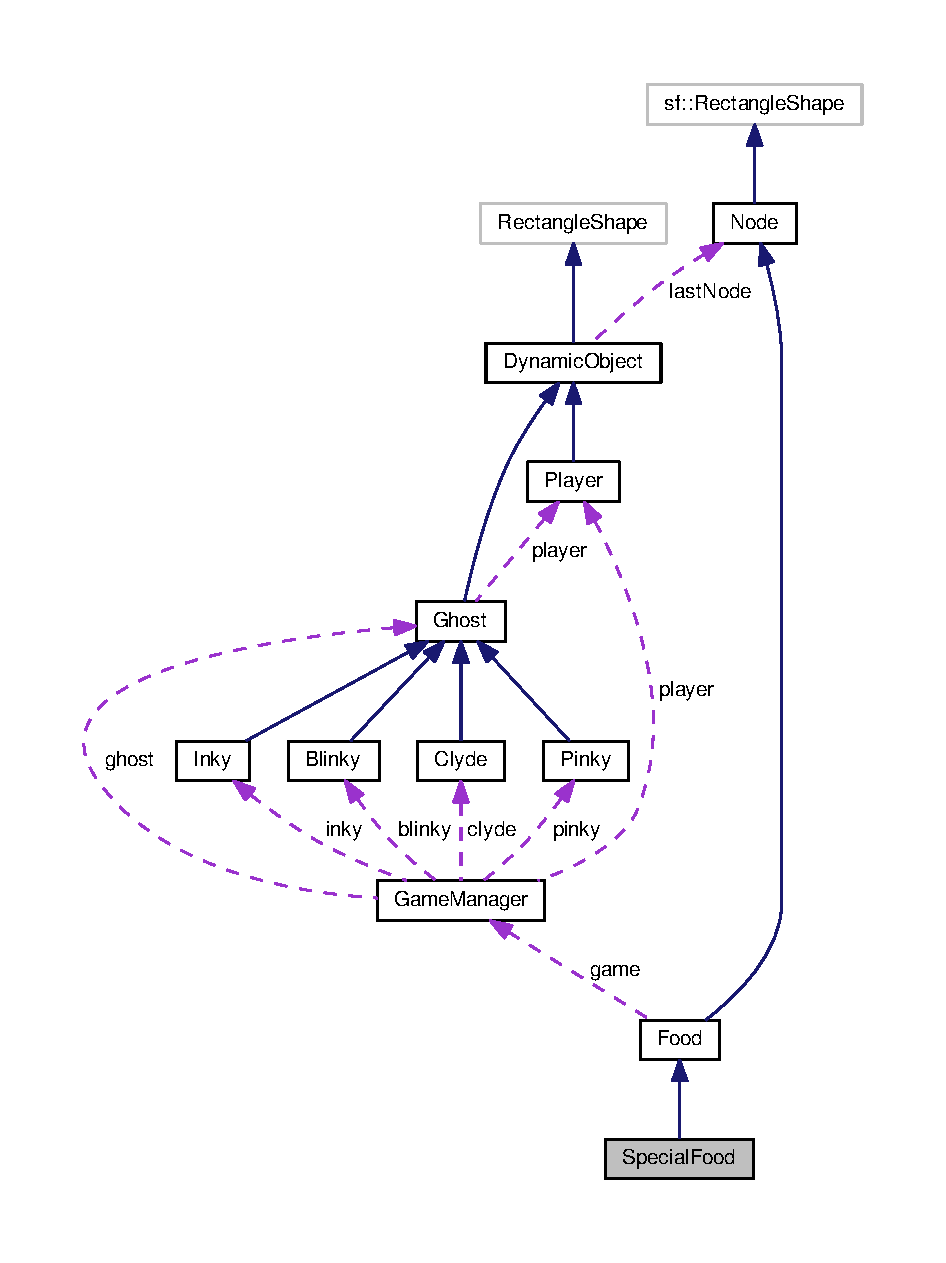
\includegraphics[width=350pt]{classSpecialFood__coll__graph}
\end{center}
\end{figure}
\subsection*{Public Member Functions}
\begin{DoxyCompactItemize}
\item 
\mbox{\Hypertarget{classSpecialFood_a1a6213e08538231651bd423f2563eb6f}\label{classSpecialFood_a1a6213e08538231651bd423f2563eb6f}} 
{\bfseries Special\+Food} (sf\+::\+Vector2f vector, bool u, bool d, bool l, bool r)
\end{DoxyCompactItemize}
\subsection*{Additional Inherited Members}


\subsection{Detailed Description}
T\+O\+DO. 

The documentation for this class was generated from the following files\+:\begin{DoxyCompactItemize}
\item 
Engine/Special\+Food.\+h\item 
Engine/Special\+Food.\+cpp\end{DoxyCompactItemize}

\hypertarget{classTunnel}{}\section{Tunnel Class Reference}
\label{classTunnel}\index{Tunnel@{Tunnel}}


Reprezentuje węzeł, który przenosi odwiedzający go obiekt do drugiego tunelu.  




{\ttfamily \#include $<$Tunnel.\+h$>$}



Inheritance diagram for Tunnel\+:\nopagebreak
\begin{figure}[H]
\begin{center}
\leavevmode
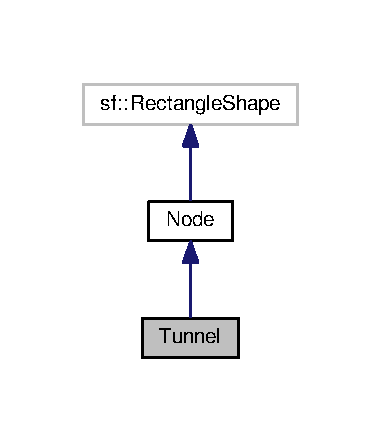
\includegraphics[width=183pt]{classTunnel__inherit__graph}
\end{center}
\end{figure}


Collaboration diagram for Tunnel\+:\nopagebreak
\begin{figure}[H]
\begin{center}
\leavevmode
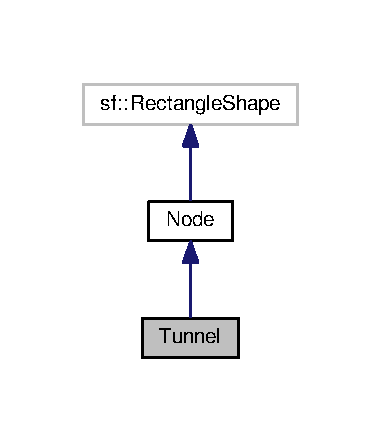
\includegraphics[width=183pt]{classTunnel__coll__graph}
\end{center}
\end{figure}
\subsection*{Public Member Functions}
\begin{DoxyCompactItemize}
\item 
\mbox{\Hypertarget{classTunnel_aec0254581076e1ea6161453e14ba7c7b}\label{classTunnel_aec0254581076e1ea6161453e14ba7c7b}} 
{\bfseries Tunnel} (sf\+::\+Vector2f vector, bool u, bool d, bool l, bool r)
\item 
\mbox{\Hypertarget{classTunnel_af17955c4f2d0bf4ff7a3cf6d00d02660}\label{classTunnel_af17955c4f2d0bf4ff7a3cf6d00d02660}} 
void \hyperlink{classTunnel_af17955c4f2d0bf4ff7a3cf6d00d02660}{visit} ()
\begin{DoxyCompactList}\small\item\em Przenosi obiekty znajdujące sie w tym węźle do drugiego tunelu. \end{DoxyCompactList}\end{DoxyCompactItemize}
\subsection*{Public Attributes}
\begin{DoxyCompactItemize}
\item 
\mbox{\Hypertarget{classTunnel_aba117d6f2bc79be7fa3d86ec121a16c3}\label{classTunnel_aba117d6f2bc79be7fa3d86ec121a16c3}} 
std\+::vector$<$ \hyperlink{classDynamicObject}{Dynamic\+Object} $\ast$ $>$ {\bfseries objects}
\item 
\mbox{\Hypertarget{classTunnel_a0dc4271e155fb13ca1eccee6eb8eaa2f}\label{classTunnel_a0dc4271e155fb13ca1eccee6eb8eaa2f}} 
Dynamic\+Object\+::\+Direction {\bfseries direction}
\end{DoxyCompactItemize}


\subsection{Detailed Description}
Reprezentuje węzeł, który przenosi odwiedzający go obiekt do drugiego tunelu. 

The documentation for this class was generated from the following files\+:\begin{DoxyCompactItemize}
\item 
Engine/Tunnel.\+h\item 
Engine/Tunnel.\+cpp\end{DoxyCompactItemize}

\hypertarget{classWallsGenerator}{}\section{Walls\+Generator Class Reference}
\label{classWallsGenerator}\index{Walls\+Generator@{Walls\+Generator}}


Klasa ma na celu utworzenie zbioru punktów, które po połączeniu mają reprezentować ściany tuneli. Schemat ścian definiowany jest w metodzie initialize\+Walls\+Scheme() w pliku Walls\+Generator.\+cpp.  




{\ttfamily \#include $<$Walls\+Generator.\+h$>$}

\subsection*{Public Member Functions}
\begin{DoxyCompactItemize}
\item 
\hyperlink{classWallsGenerator_ae1cfcd3b678f1de130b146dfcee08d68}{Walls\+Generator} (sf\+::\+Vertex\+Array \&walls, sf\+::\+Vector2f left\+Up\+Corner)
\end{DoxyCompactItemize}


\subsection{Detailed Description}
Klasa ma na celu utworzenie zbioru punktów, które po połączeniu mają reprezentować ściany tuneli. Schemat ścian definiowany jest w metodzie initialize\+Walls\+Scheme() w pliku Walls\+Generator.\+cpp. 

\subsection{Constructor \& Destructor Documentation}
\mbox{\Hypertarget{classWallsGenerator_ae1cfcd3b678f1de130b146dfcee08d68}\label{classWallsGenerator_ae1cfcd3b678f1de130b146dfcee08d68}} 
\index{Walls\+Generator@{Walls\+Generator}!Walls\+Generator@{Walls\+Generator}}
\index{Walls\+Generator@{Walls\+Generator}!Walls\+Generator@{Walls\+Generator}}
\subsubsection{\texorpdfstring{Walls\+Generator()}{WallsGenerator()}}
{\footnotesize\ttfamily Walls\+Generator\+::\+Walls\+Generator (\begin{DoxyParamCaption}\item[{sf\+::\+Vertex\+Array \&}]{walls,  }\item[{sf\+::\+Vector2f}]{left\+Up\+Corner }\end{DoxyParamCaption})}

wypełnia wektor walls punktami, które po połączeniu utworzą ściany tuneli 
\begin{DoxyParams}{Parameters}
{\em walls} & pusty wektor \\
\hline
{\em left\+Up\+Corner} & Położenie górnego, lewego rogu wygenerowanego schematu ścian tuneli \\
\hline
\end{DoxyParams}


The documentation for this class was generated from the following files\+:\begin{DoxyCompactItemize}
\item 
Walls\+Generator.\+h\item 
Walls\+Generator.\+cpp\end{DoxyCompactItemize}

%--- End generated contents ---

% Index
\backmatter
\newpage
\phantomsection
\clearemptydoublepage
\addcontentsline{toc}{chapter}{Index}
\printindex

\end{document}
